\chapter{Chapter 2 appendix}
\section{Nucleoside and nucleobase quantification}
blaa


% isotope_enrichment folder (under lab-work)

% IncuCyte_vs_Flow_ATF4-reporter_01-13-22

















\section{Packed cell volume is an overestimate in common cancer cell lines}
\label{app_ch2_cell_vol}
This is an abridged version of the method and results in Engstrom et al. 2021 \cite{Engstrom2021-az}.

Originally developed to determine the volume of red cells in blood, or hematocrit, packed cell volume (PCV) measurements have more recently also been used to determine the volume of adherent cell lines for conversion of intracellular metabolite quantities into concentrations \cite{Park2016-ap, Liu2018-it, Yang2020-fs, Ghergurovich2020-nb}.
Another way of determining cell volume is using the Coulter principle which relates particle volume to the change in electrical impedance as the particle passes through an aperture.
For blood, PCV is a reliable measurement, proportional to the cell volume determined using the Coulter principle \cite{Carter1968-xy, Bull2001-xb}; however, this assumption has not been tested for the diverse set of cell lines used for cell culturing.

We compared PCV with Coulter counter-based cell volume measurements for five cell lines and found that the spin protocol provided by the PCV tube manufacturer (2,500 g for 1 min) lead to an overestimate of cell volume compared to Coulter-based measurements.
We hypothesized that this discrepancy is related to incomplete cell packing and that packing efficiency is negatively impacted by ``sticky'' extracellular matrix proteins found abundantly on adherent cells.
This was tested with five different cell lines by increasing the centrifugation speed and time (figure \ref{fig:app_ch2:CCvsPCV}).
The results showed that PCV measurements at the lowest centrifugation speed were overestimates of cell volume compared to Coulter-based measurements for all cell lines.
Adherent cells had the largest volume discrepancy.
PCV measurements decreased with increasing centrifugation speed and time and approached the Coulter-based volume.

In summary, the results indicate that PCV consistently overestimates cell volume compared to measurements using a Coulter counter.
This overestimate in PCV is likely due to incomplete packing, which is particularly problematic for adherent cell lines.
Therefore, it is advisable for future studies relying on accurate cell volume measurements to use the Coulter principle for cell volume measurement.

\begin{figure}[ht]
    \centering
    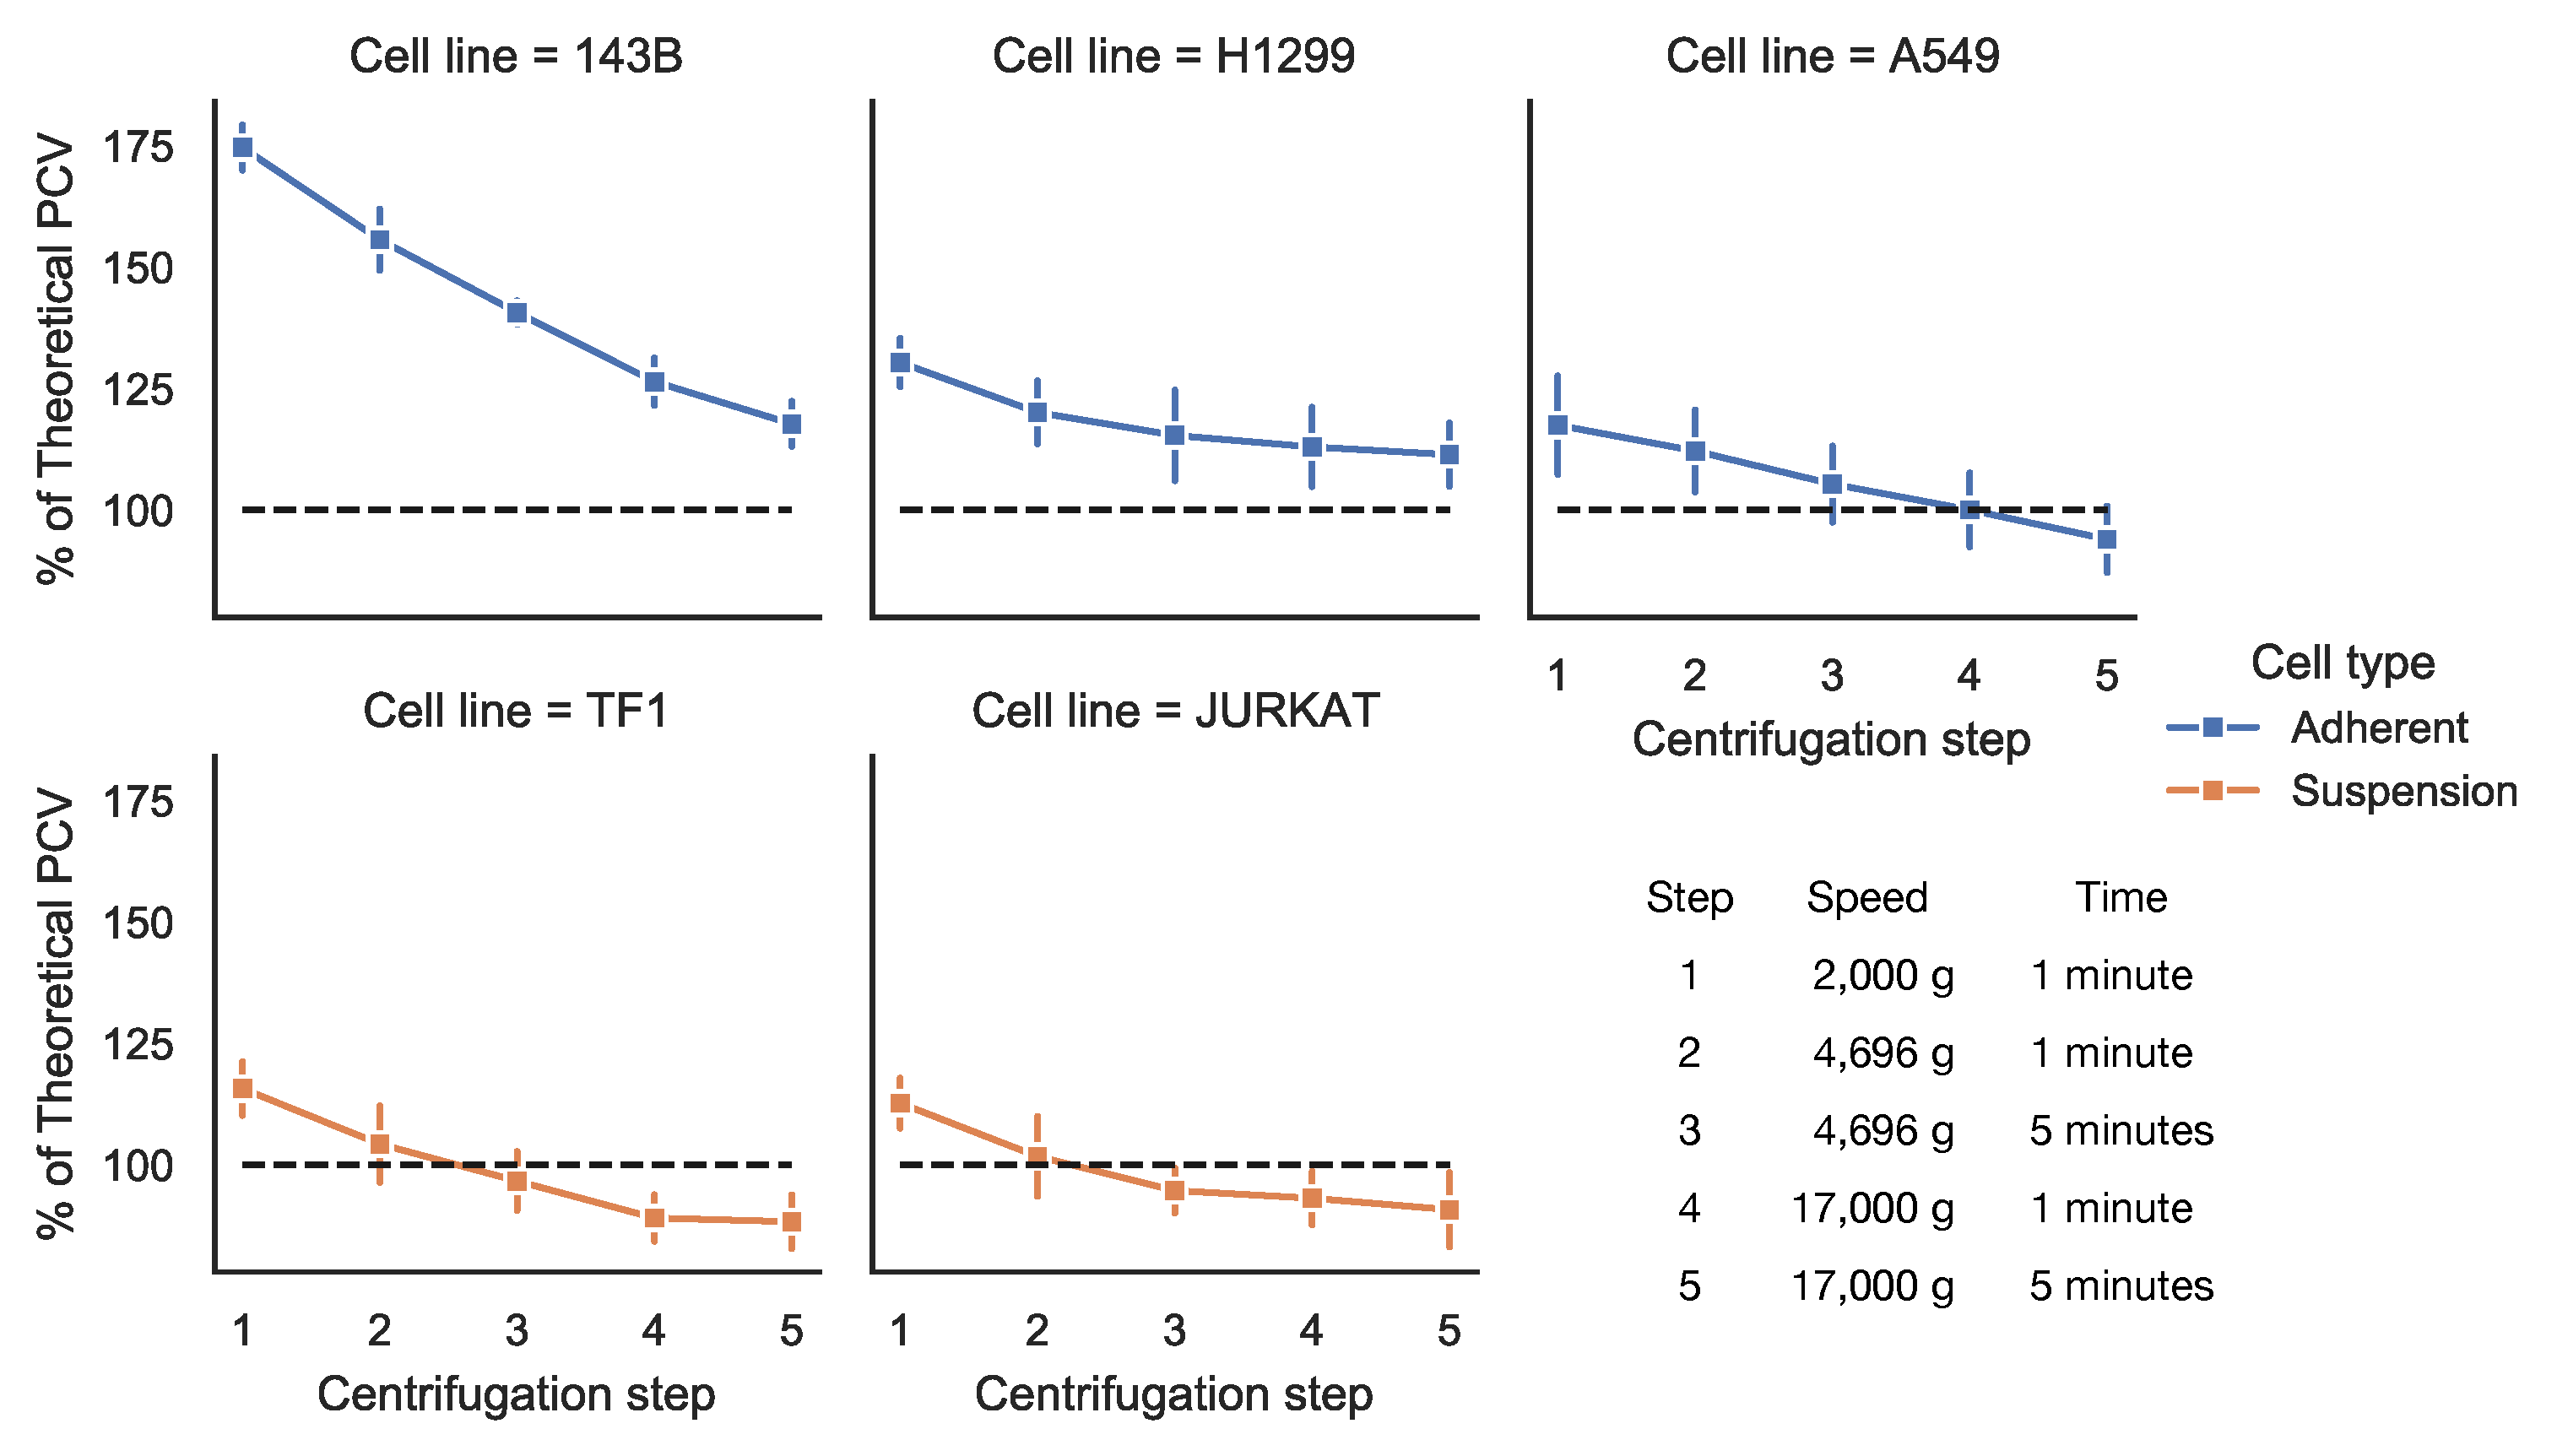
\includegraphics[width=0.99\textwidth]{figures/chap2/app/CCvsPCV.pdf}
    \caption[Packed cell volume vs. Coulter counter]{
    Packed cell volume (PCV) compared to the theoretical volume as determined by a Coulter counter (Multisizer 4 ).
    }
    \label{fig:app_ch2:CCvsPCV}
\end{figure}






\section{Aspartate to proliferation curves}



\begin{figure}
    \centering
    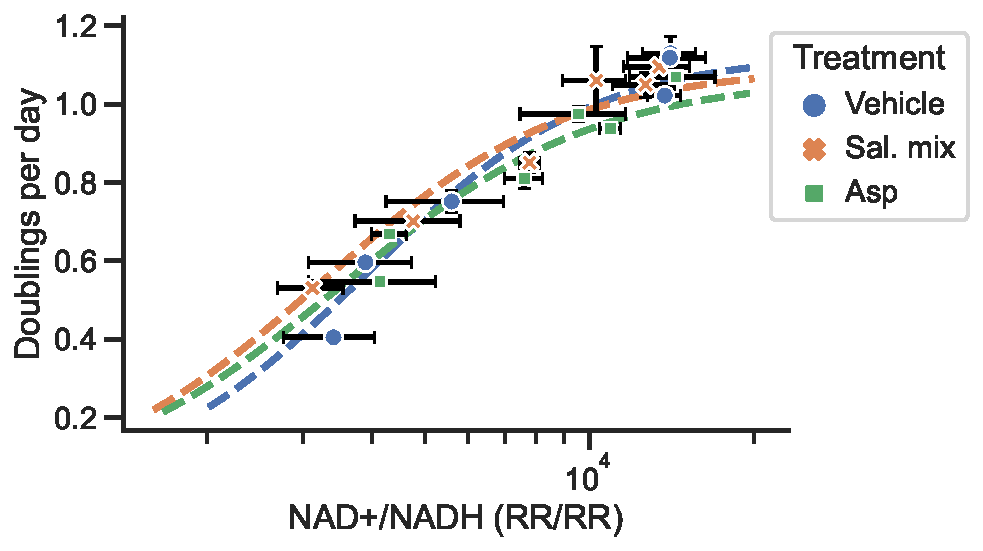
\includegraphics[width=0.7\textwidth]{figures/chap2/app/H1299_Rot_NAD_vs_prlfr_noPyr.pdf}
    \caption[ggggg]{
    \NAD{}/NADH ratio for same data as in figure \ref{fig:ch2:H1299_Rot_Asp_vs_prlfr}.
    }
    \label{fig:app_ch2:H1299_Rot_NAD_vs_prlfr}
\end{figure}


\begin{figure}
     \centering
     \begin{subfigure}[b]{0.49\textwidth}
         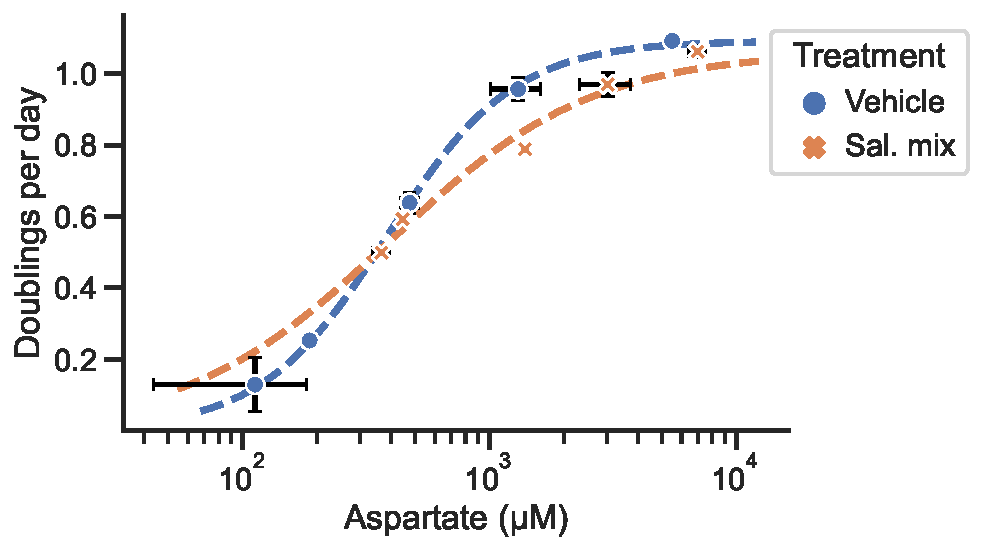
\includegraphics[width=\textwidth]{figures/chap2/app/H1299_Met_Asp_vs_prlfr.pdf}
         \caption{}
         \label{fig:app_ch2:H1299_Met_Asp_vs_prlfr}
     \end{subfigure}
     \hfill
     \begin{subfigure}[b]{0.49\textwidth}
         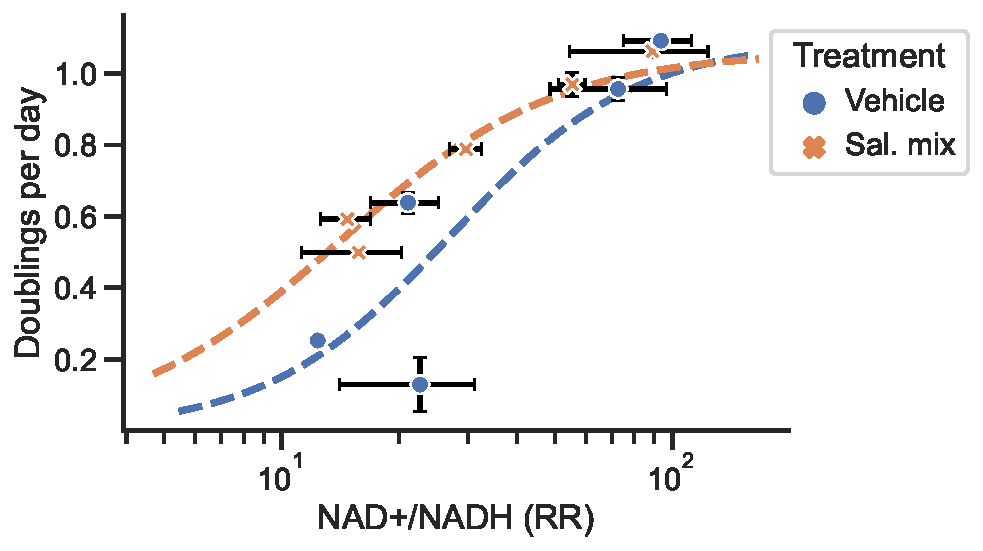
\includegraphics[width=\textwidth]{figures/chap2/app/H1299_Met_NAD_vs_prlfr.pdf}
         \caption{}
         \label{fig:app_ch2:H1299_Met_NAD_vs_prlfr}
     \end{subfigure}
        \caption[hhhh]{
        Aspartate concentration at 50\% proliferation is 390 µM for both Vehicle and Sal. mix treatments.
        }
        \label{fig:app_ch2:H1299_asp_prlfr_met}
\end{figure}



\begin{figure}
     \centering
     \begin{subfigure}[b]{0.49\textwidth}
         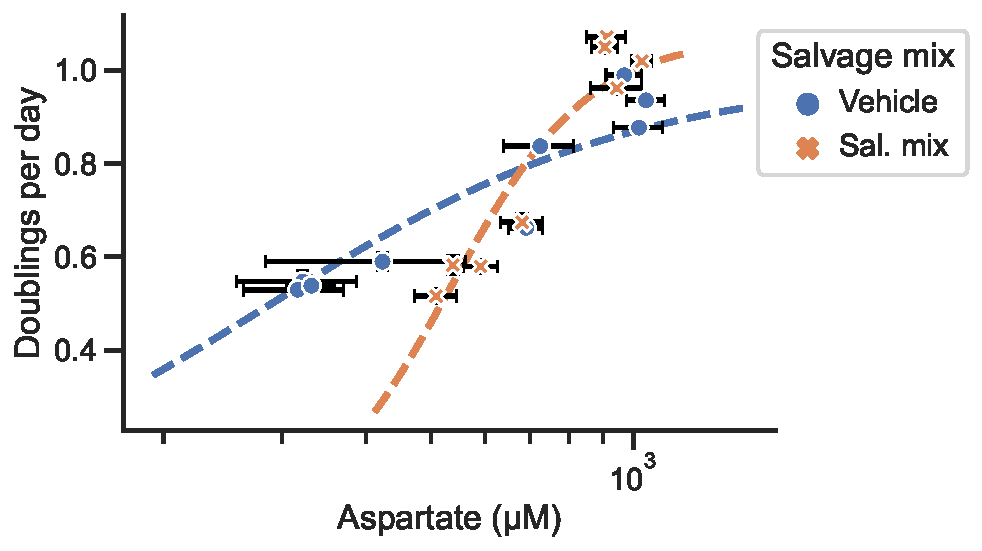
\includegraphics[width=\textwidth]{figures/chap2/app/HCT116_Met_Asp_vs_prlfr.pdf}
         \caption{}
         \label{fig:app_ch2:HCT116_Met_Asp_vs_prlfr}
     \end{subfigure}
     \hfill
     \begin{subfigure}[b]{0.49\textwidth}
         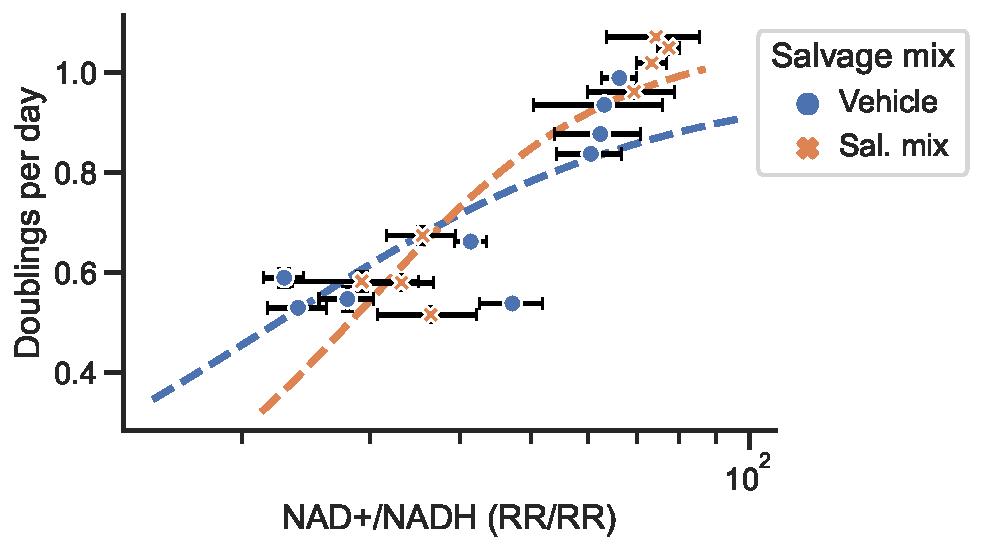
\includegraphics[width=\textwidth]{figures/chap2/app/HCT116_Met_NAD_vs_prlfr.pdf}
         \caption{}
         \label{fig:app_ch2:HCT116_Met_NAD_vs_prlfr}
     \end{subfigure}
        \caption[hhhh]{
        Aspartate concentration at 50\% proliferation is 290 and 530 µM for Vehicle and Sal. mix treatments, respectively.
        }
        \label{fig:app_ch2:HCT116_asp_prlfr_met}
\end{figure}



\begin{figure}
    \centering
    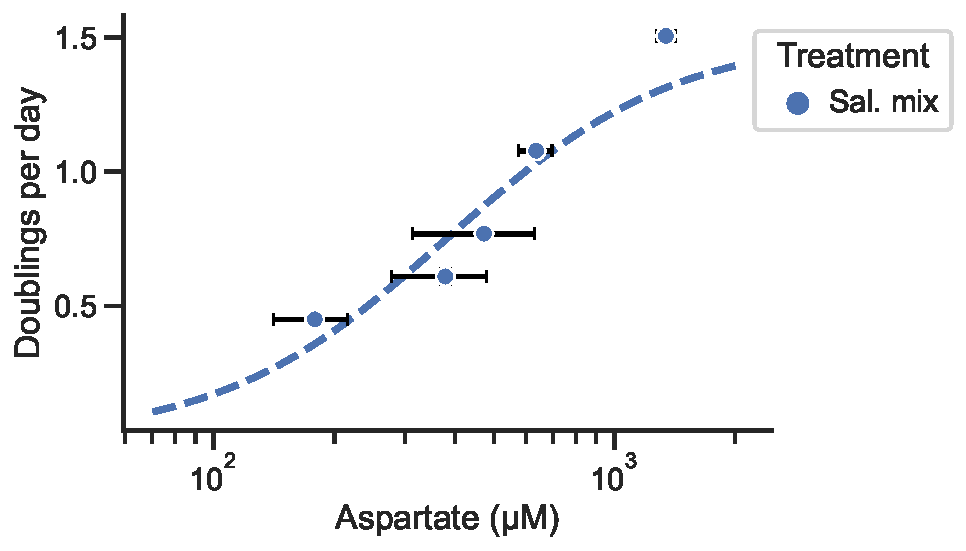
\includegraphics[width=0.49\textwidth]{figures/chap2/app/143B_Met_Asp_vs_prlfr.pdf}
    \caption[ggggg]{
    Aspartate concentration at 50\% proliferation is 380 µM for Sal. mix treated cells.
    }
    \label{fig:app_ch2:143B_Met_Asp_vs_prlfr}
\end{figure}









\section{Nucleoside and nucleobase quantification}

\begin{figure}[!ht]
    \captionsetup{labelformat=empty}
    \centering
    \begin{subfigure}[b]{0.68\textwidth}
        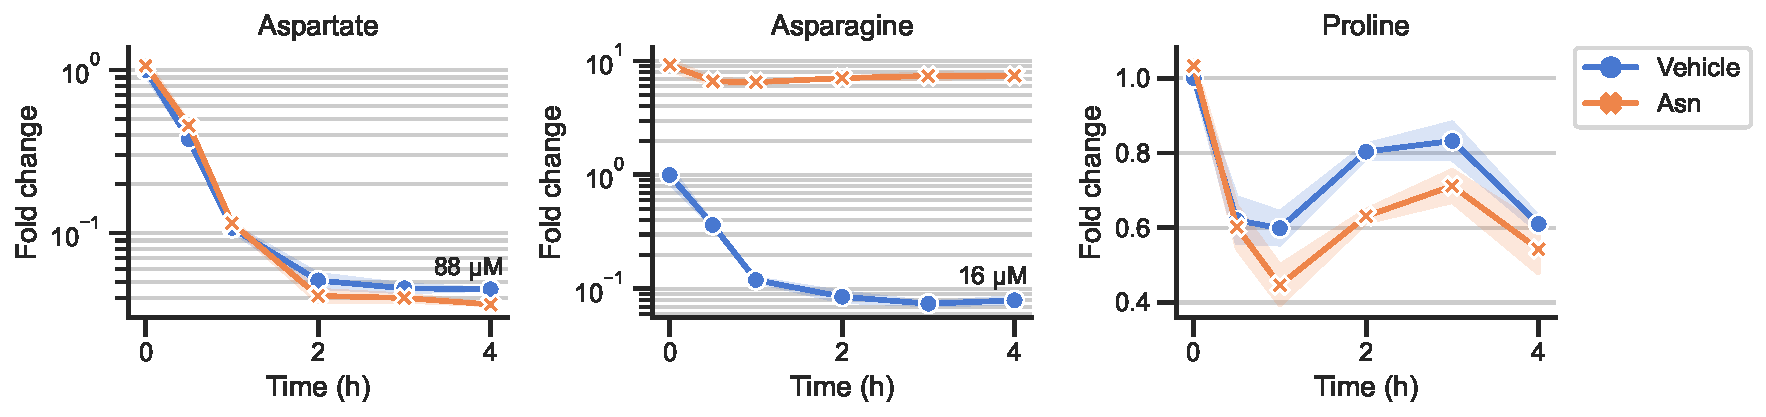
\includegraphics[width=\textwidth]{figures/chap2/app/HT1080_Anti_AA.pdf}
        \caption{Amino acids}
        \label{fig:app_ch2:HT1080_Anti_AA}
    \end{subfigure}
    \hfill
    \begin{subfigure}[b]{0.45\textwidth}
        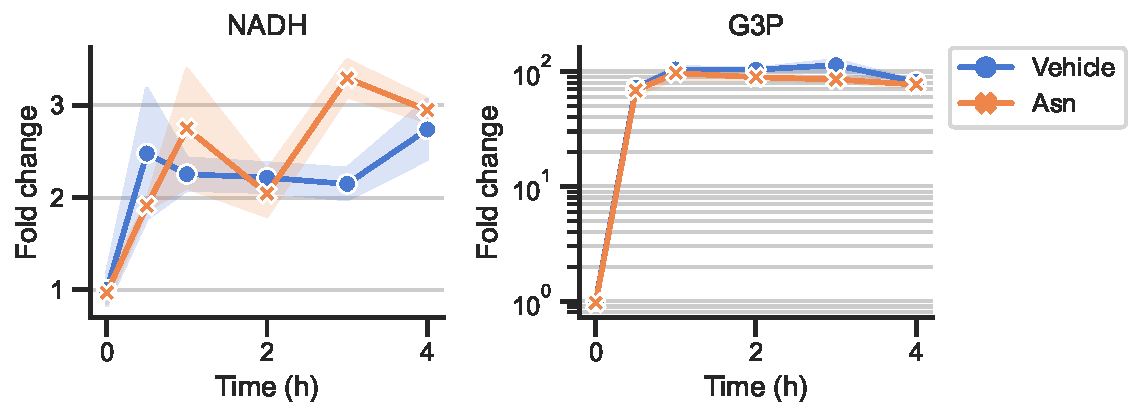
\includegraphics[width=\textwidth]{figures/chap2/app/HT1080_Anti_rd.pdf}
        \caption{Redox metabolites}
        \label{fig:app_ch2:HT1080_Anti_rd}
    \end{subfigure}
    \hfill
    \begin{subfigure}[b]{0.9\textwidth}
        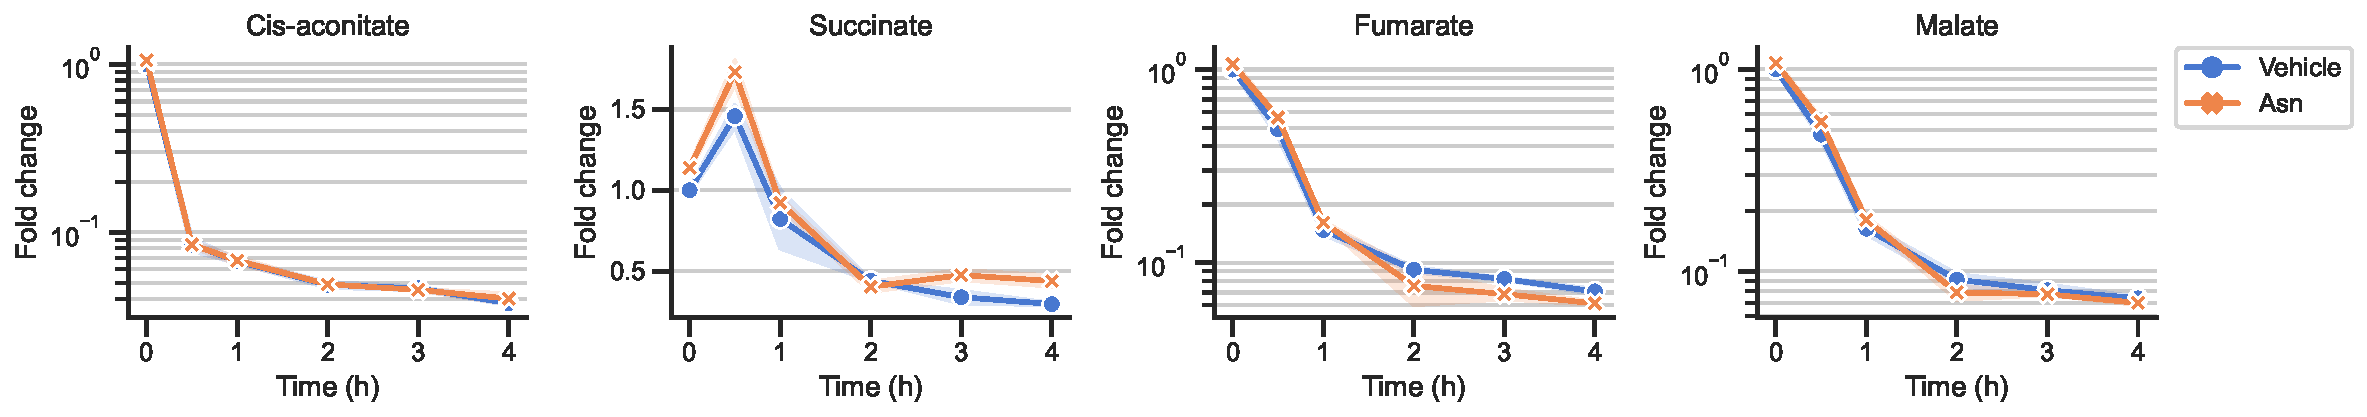
\includegraphics[width=\textwidth]{figures/chap2/app/HT1080_Anti_tca.pdf}
        \caption{TCA metabolites}
        \label{fig:app_ch2:HT1080_Anti_tca}
    \end{subfigure}
    \hfill
    \begin{subfigure}[b]{0.68\textwidth}
        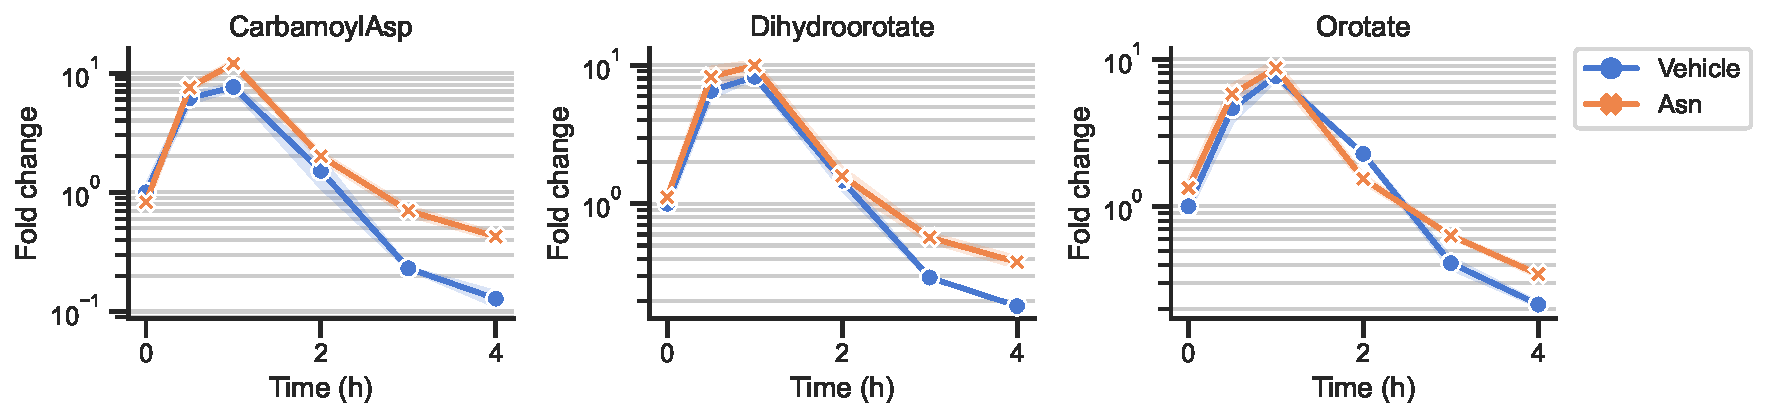
\includegraphics[width=\textwidth]{figures/chap2/app/HT1080_Anti_pyr.pdf}
        \caption{Pyrimidine metabolites}
        \label{fig:app_ch2:HT1080_Anti_pyr}
    \end{subfigure}
    \hfill
    \begin{subfigure}[b]{0.9\textwidth}
        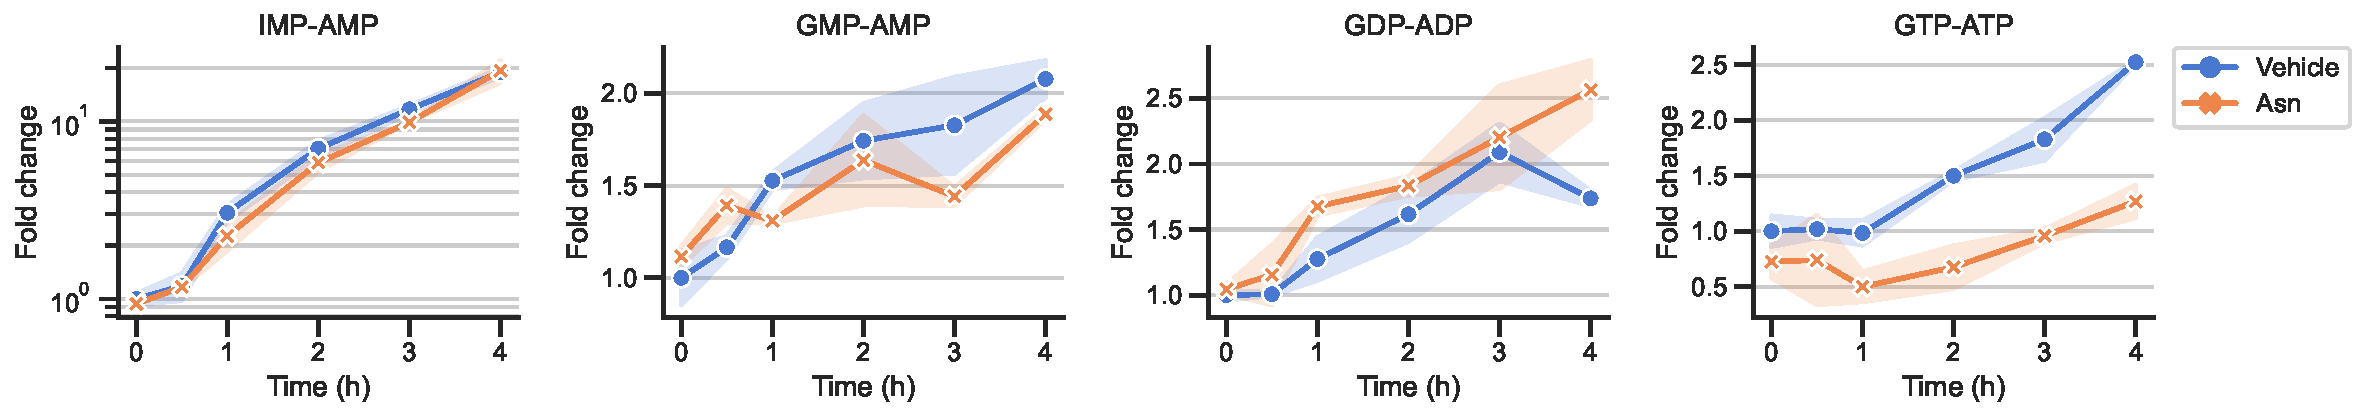
\includegraphics[width=\textwidth]{figures/chap2/app/HT1080_Anti_pur.pdf}
        \caption{Purine ratios}
        \label{fig:app_ch2:HT1080_Anti_pur}
    \end{subfigure}
    \hfill
    \caption{}
\end{figure}

\begin{figure}[!ht]
    % \captionsetup{labelformat=empty}
    \ContinuedFloat
    \centering
    \begin{subfigure}[b]{0.68\textwidth}
        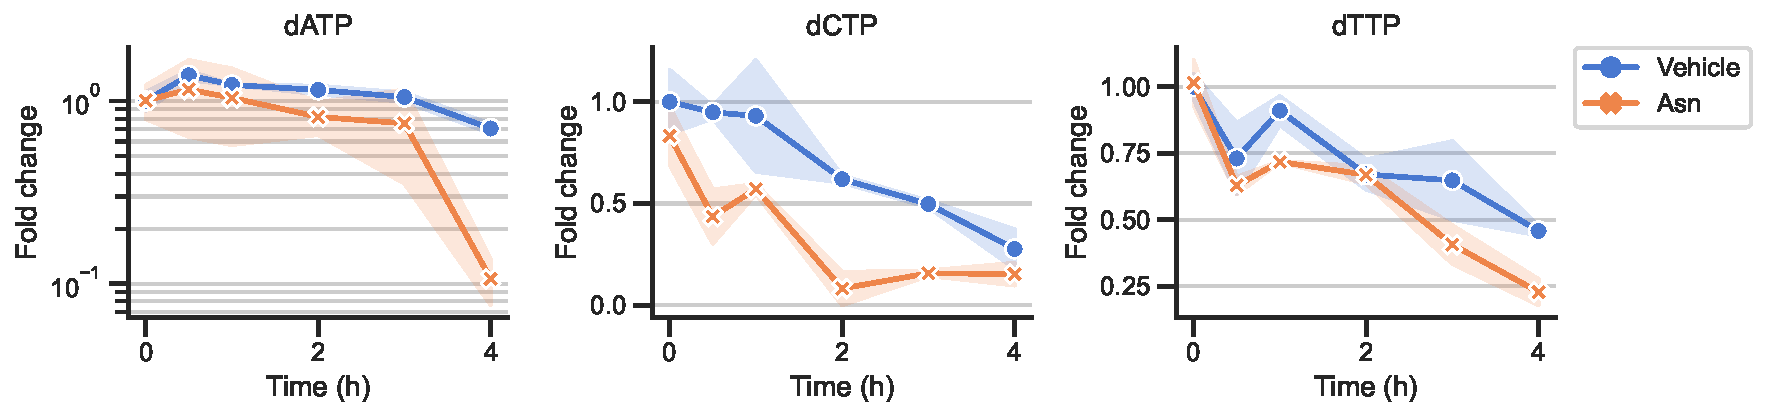
\includegraphics[width=\textwidth]{figures/chap2/app/HT1080_Anti_dntps.pdf}
        \caption{dNTPs}
        \label{fig:app_ch2:HT1080_Anti_dntps}
    \end{subfigure}
    \hfill
    \begin{subfigure}[b]{0.68\textwidth}
        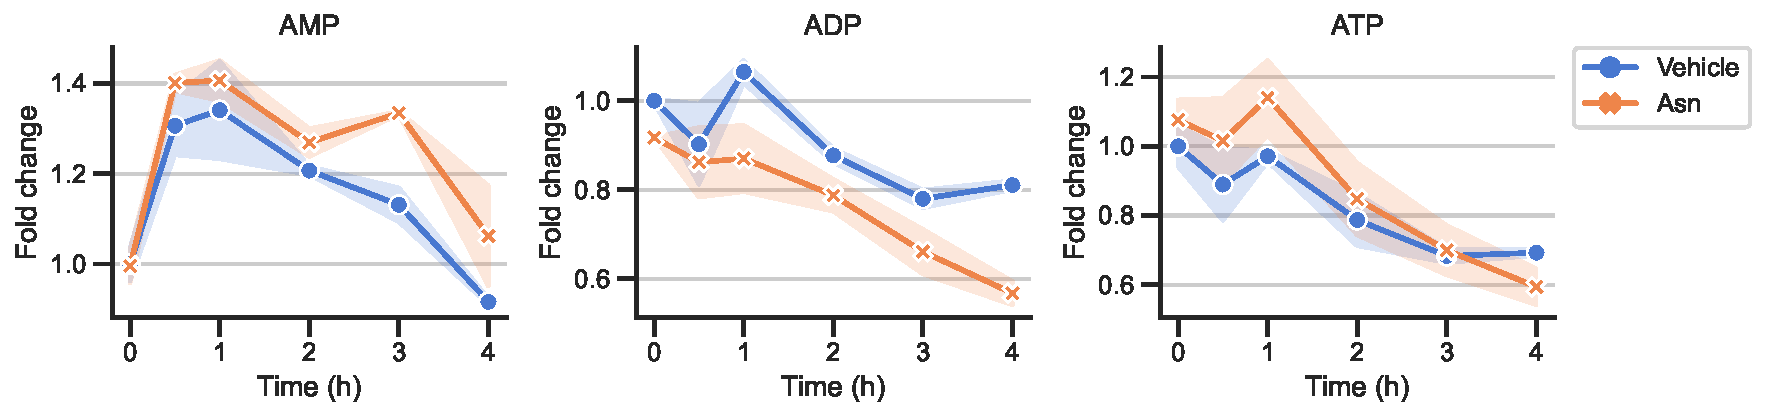
\includegraphics[width=\textwidth]{figures/chap2/app/HT1080_Anti_axp.pdf}
        \caption{AXPs}
        \label{fig:app_ch2:HT1080_Anti_axp}
    \end{subfigure}
    \hfill
    \begin{subfigure}[b]{0.68\textwidth}
        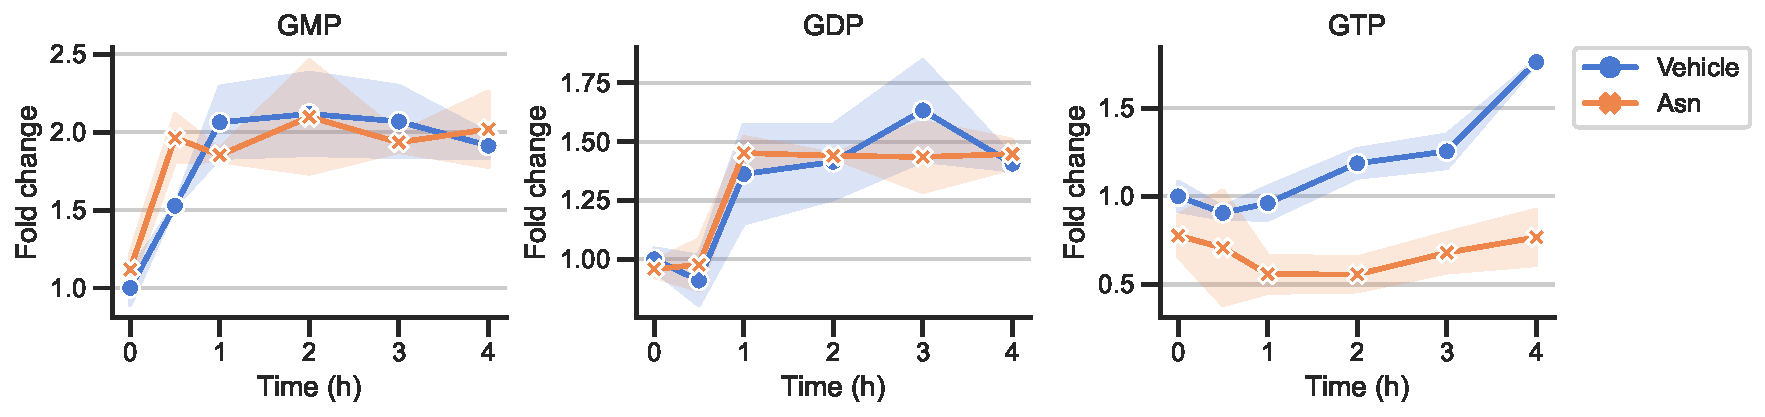
\includegraphics[width=\textwidth]{figures/chap2/app/HT1080_Anti_gxp.pdf}
        \caption{GXPs}
        \label{fig:app_ch2:HT1080_Anti_gxp}
    \end{subfigure}
    \hfill
    \begin{subfigure}[b]{0.68\textwidth}
        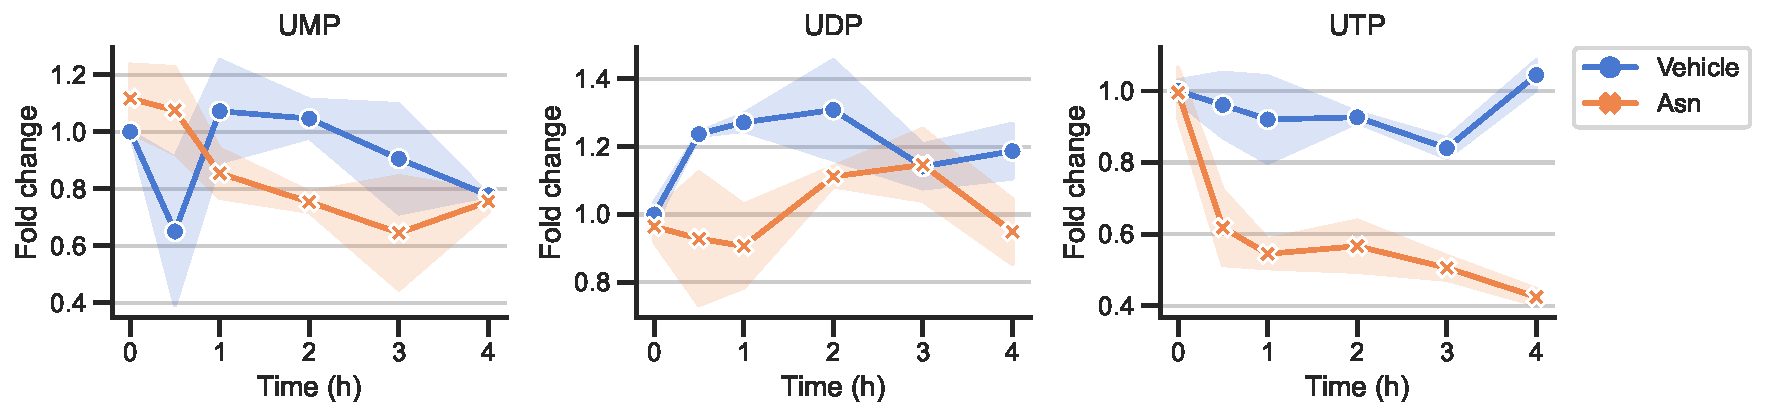
\includegraphics[width=\textwidth]{figures/chap2/app/HT1080_Anti_uxp.pdf}
        \caption{UXPs}
        \label{fig:app_ch2:HT1080_Anti_uxp}
    \end{subfigure}
    \hfill
    \begin{subfigure}[b]{0.68\textwidth}
        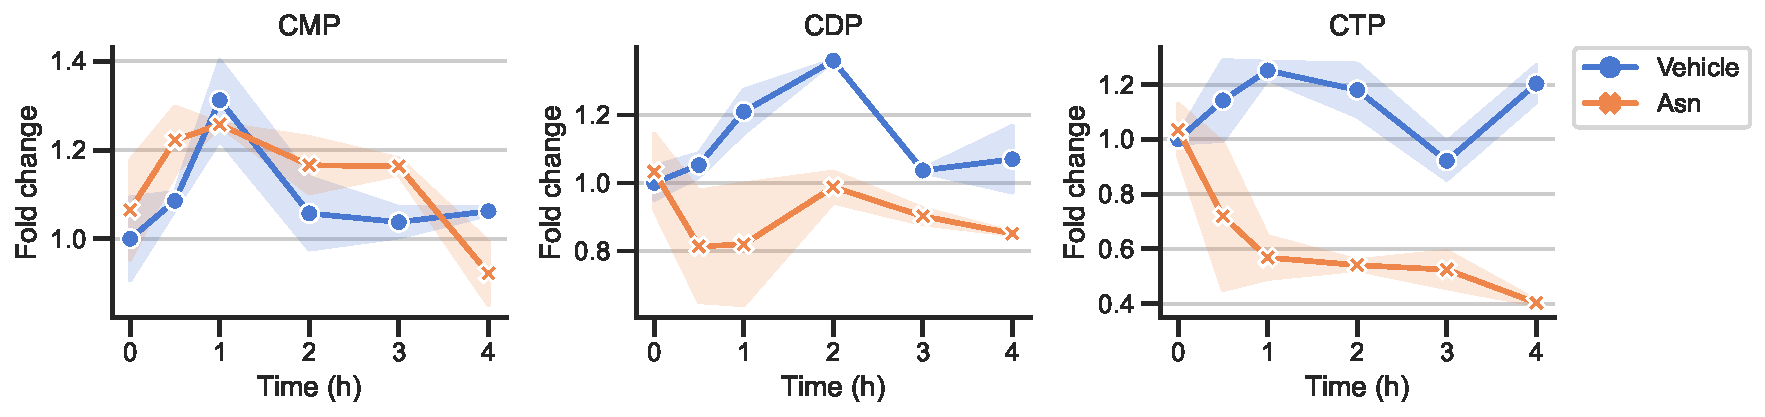
\includegraphics[width=\textwidth]{figures/chap2/app/HT1080_Anti_cxp.pdf}
        \caption{CXPs}
        \label{fig:app_ch2:HT1080_Anti_cxp}
    \end{subfigure}
    \hfill
        \caption[Metabolic changes in HT1080 after antimycin treatment]{
        Metabolic changes in HT1080 WT after antimycin (1 µM) treatment.
        From same experiment as figure \ref{fig:ch2:ISR_resc}.
        }
        \label{fig:app_ch2:HT1080_Anti_metab}
\end{figure}















\begin{figure}
    \centering
    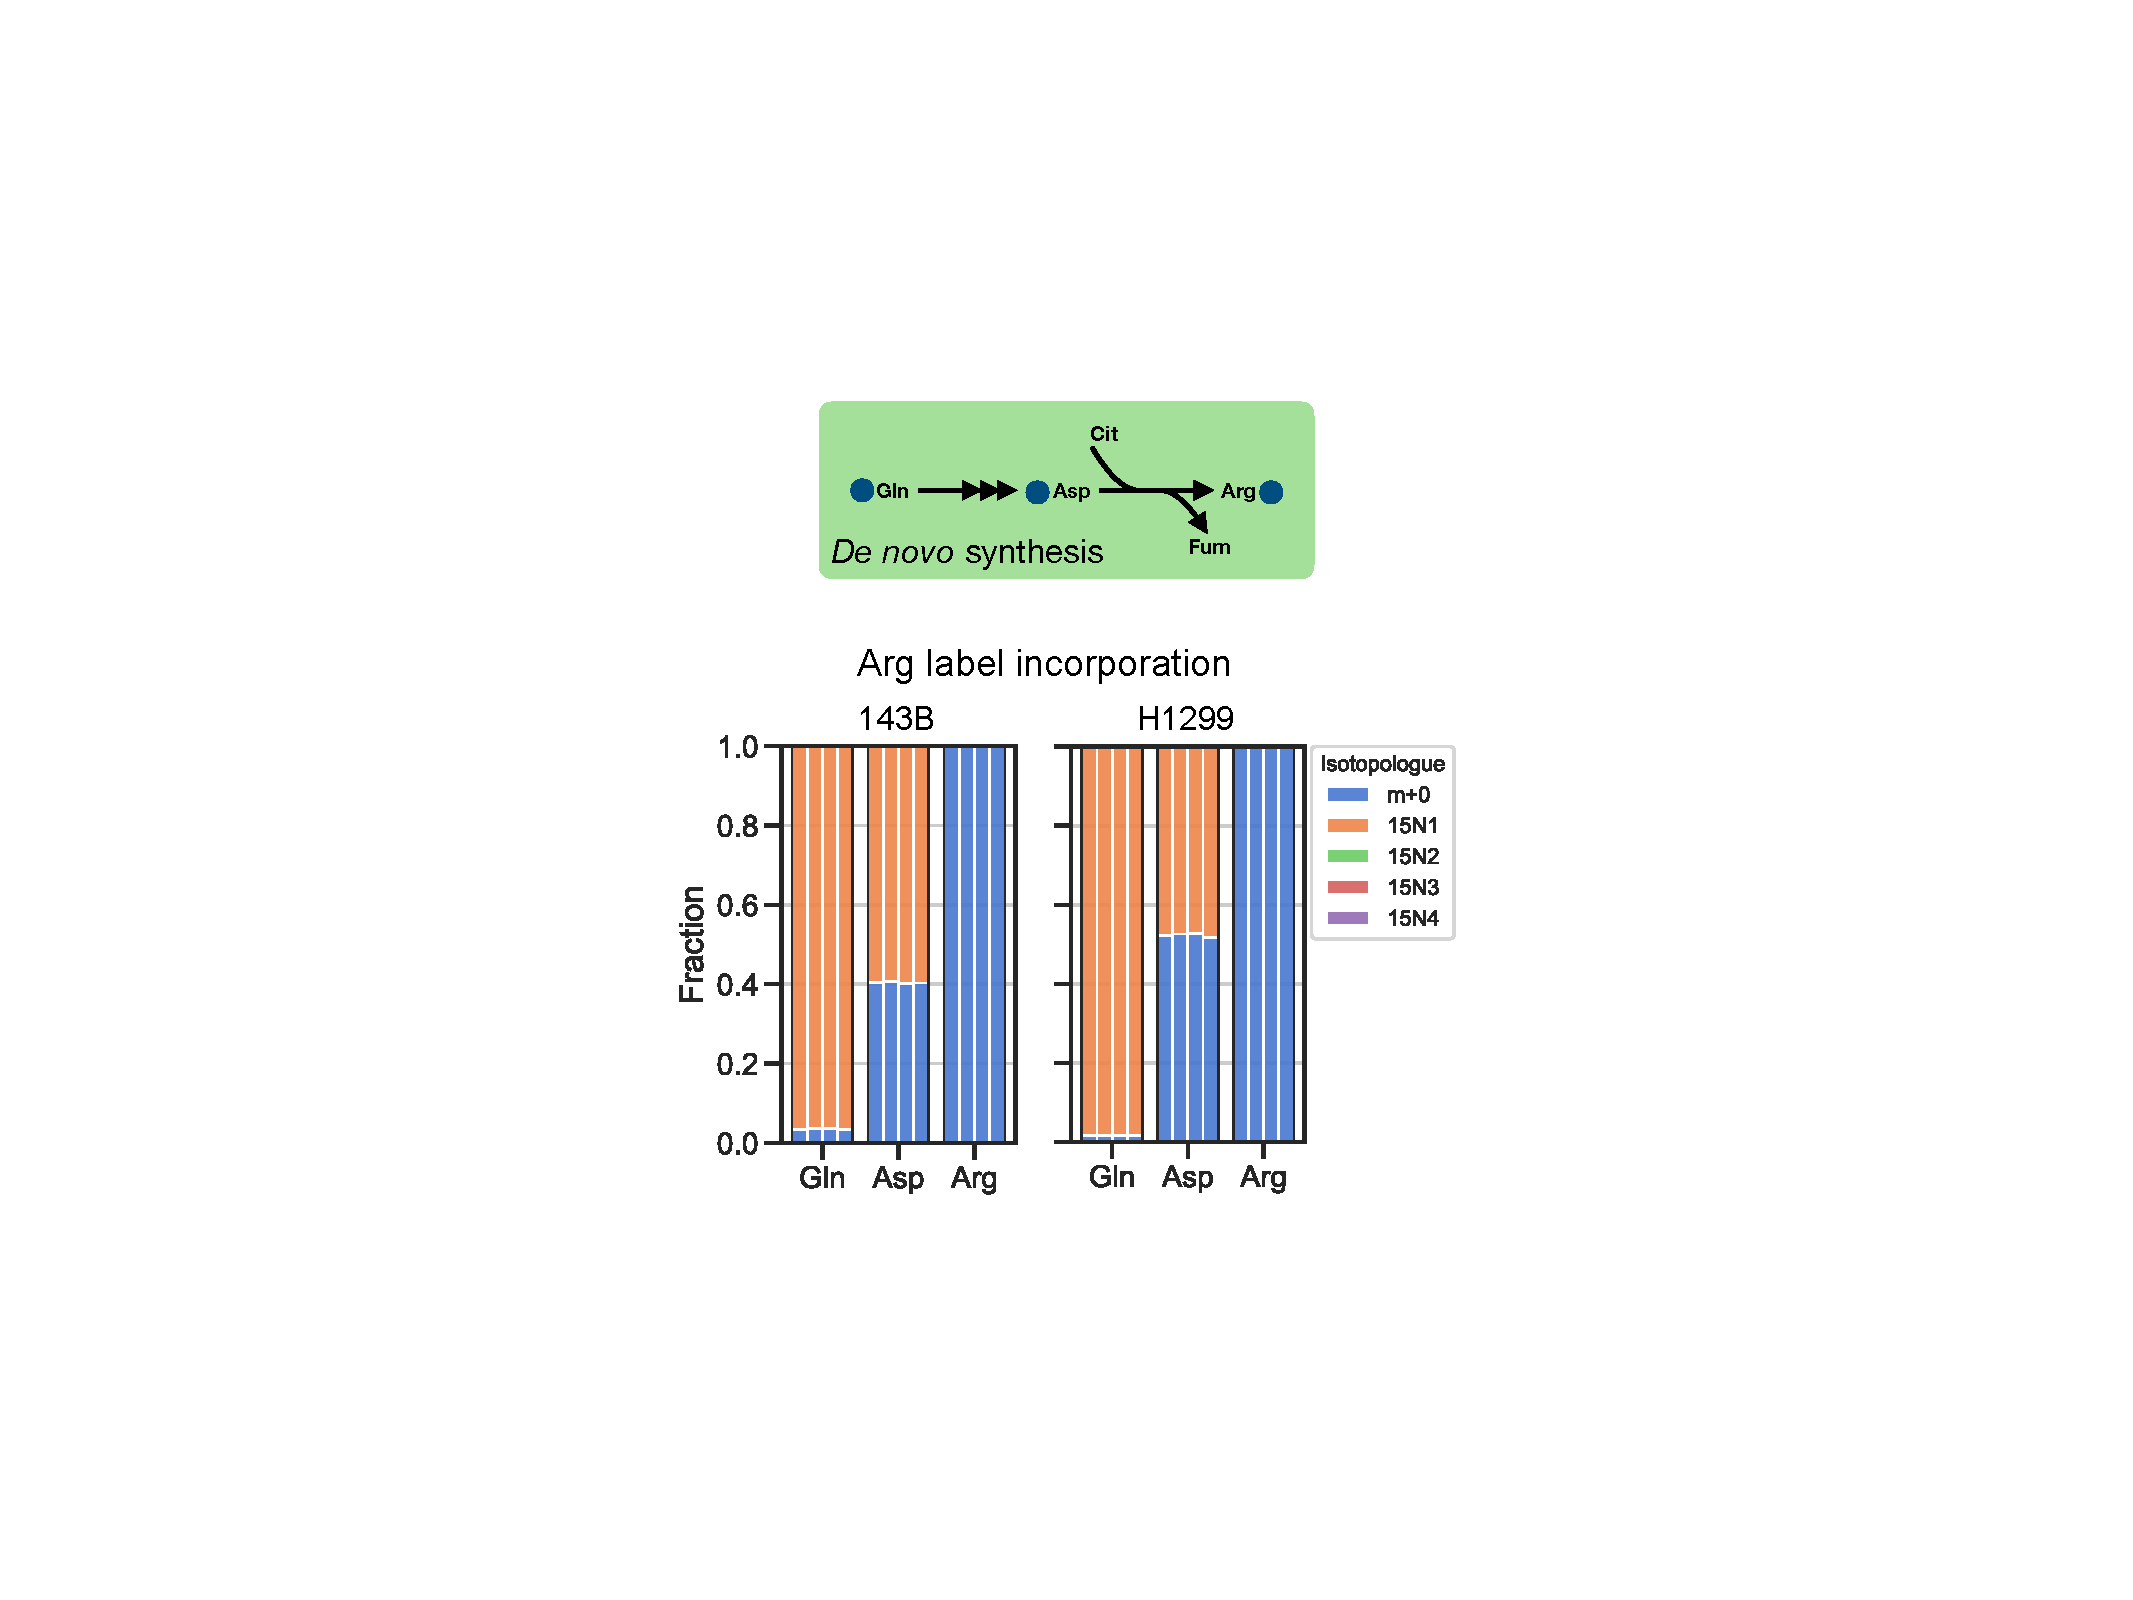
\includegraphics[width=0.45\textwidth]{figures/chap2/app/arg_syn.pdf}
    \caption[No evidence of arginine synthesis in DMEM]{
    No evidence of arginine synthesis in DMEM.
    Top diagram shows Gln alpha\=/\hNi{} label incorporation into Asp and subsequently Arg.
    Bottom isotopologue distribution shows Gln alpha\=/\hNi{} label incorporation into Gln, Asp and Arg at steady-state for cell lines 143B and H1299 grown in DMEM.
    }
    \label{fig:app_ch2:arg_syn}
\end{figure}










\begin{figure}
    \centering
    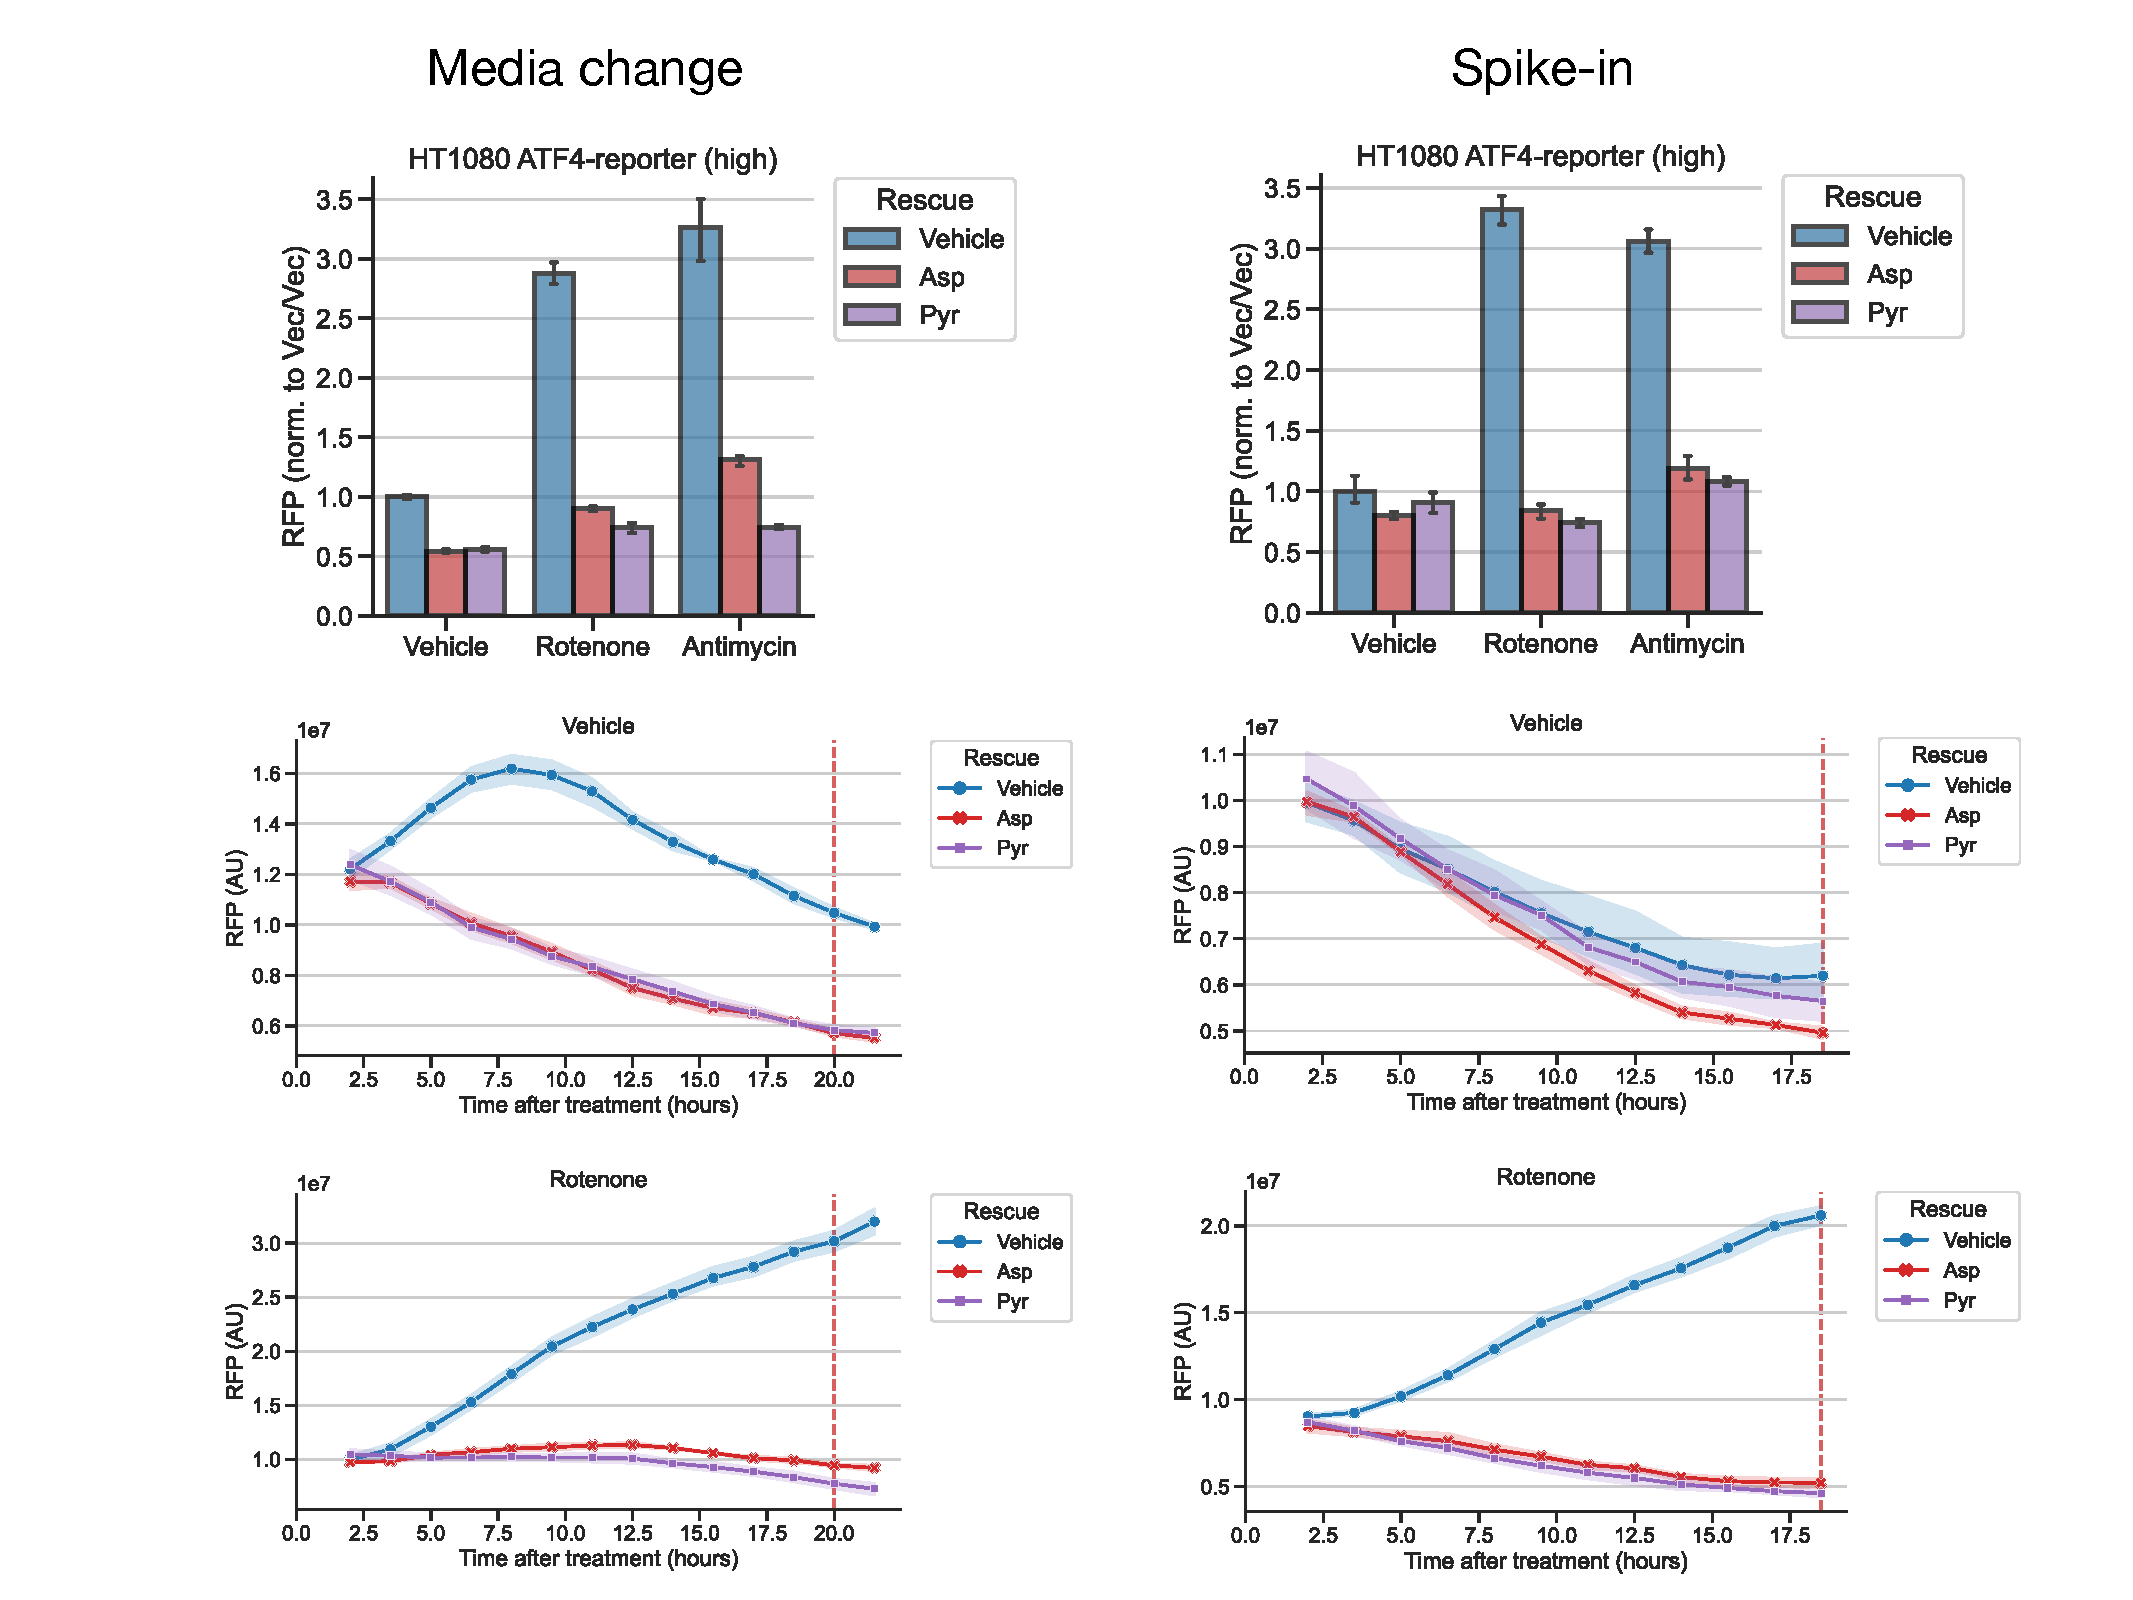
\includegraphics[width=0.95\textwidth]{figures/chap2/app/atf4_chVSsp.pdf}
    \caption[ATF4 reporter, media change vs. spike-in]{
    Mitochondrial inhibitor induced ATF4 reporter, media change vs. spike-in.
    Left column showing results from an experiment were media change was used to initiate the treatment.
    Right column showing results from an experiment were the treatment was initiated by a 10x spike-in.
    Barplots showing results at the time indicated by the red dashed line on the lineplots below.
    }
    \label{fig:app_ch2:sal_frac_conc}
\end{figure}


\begin{figure}
    \centering
    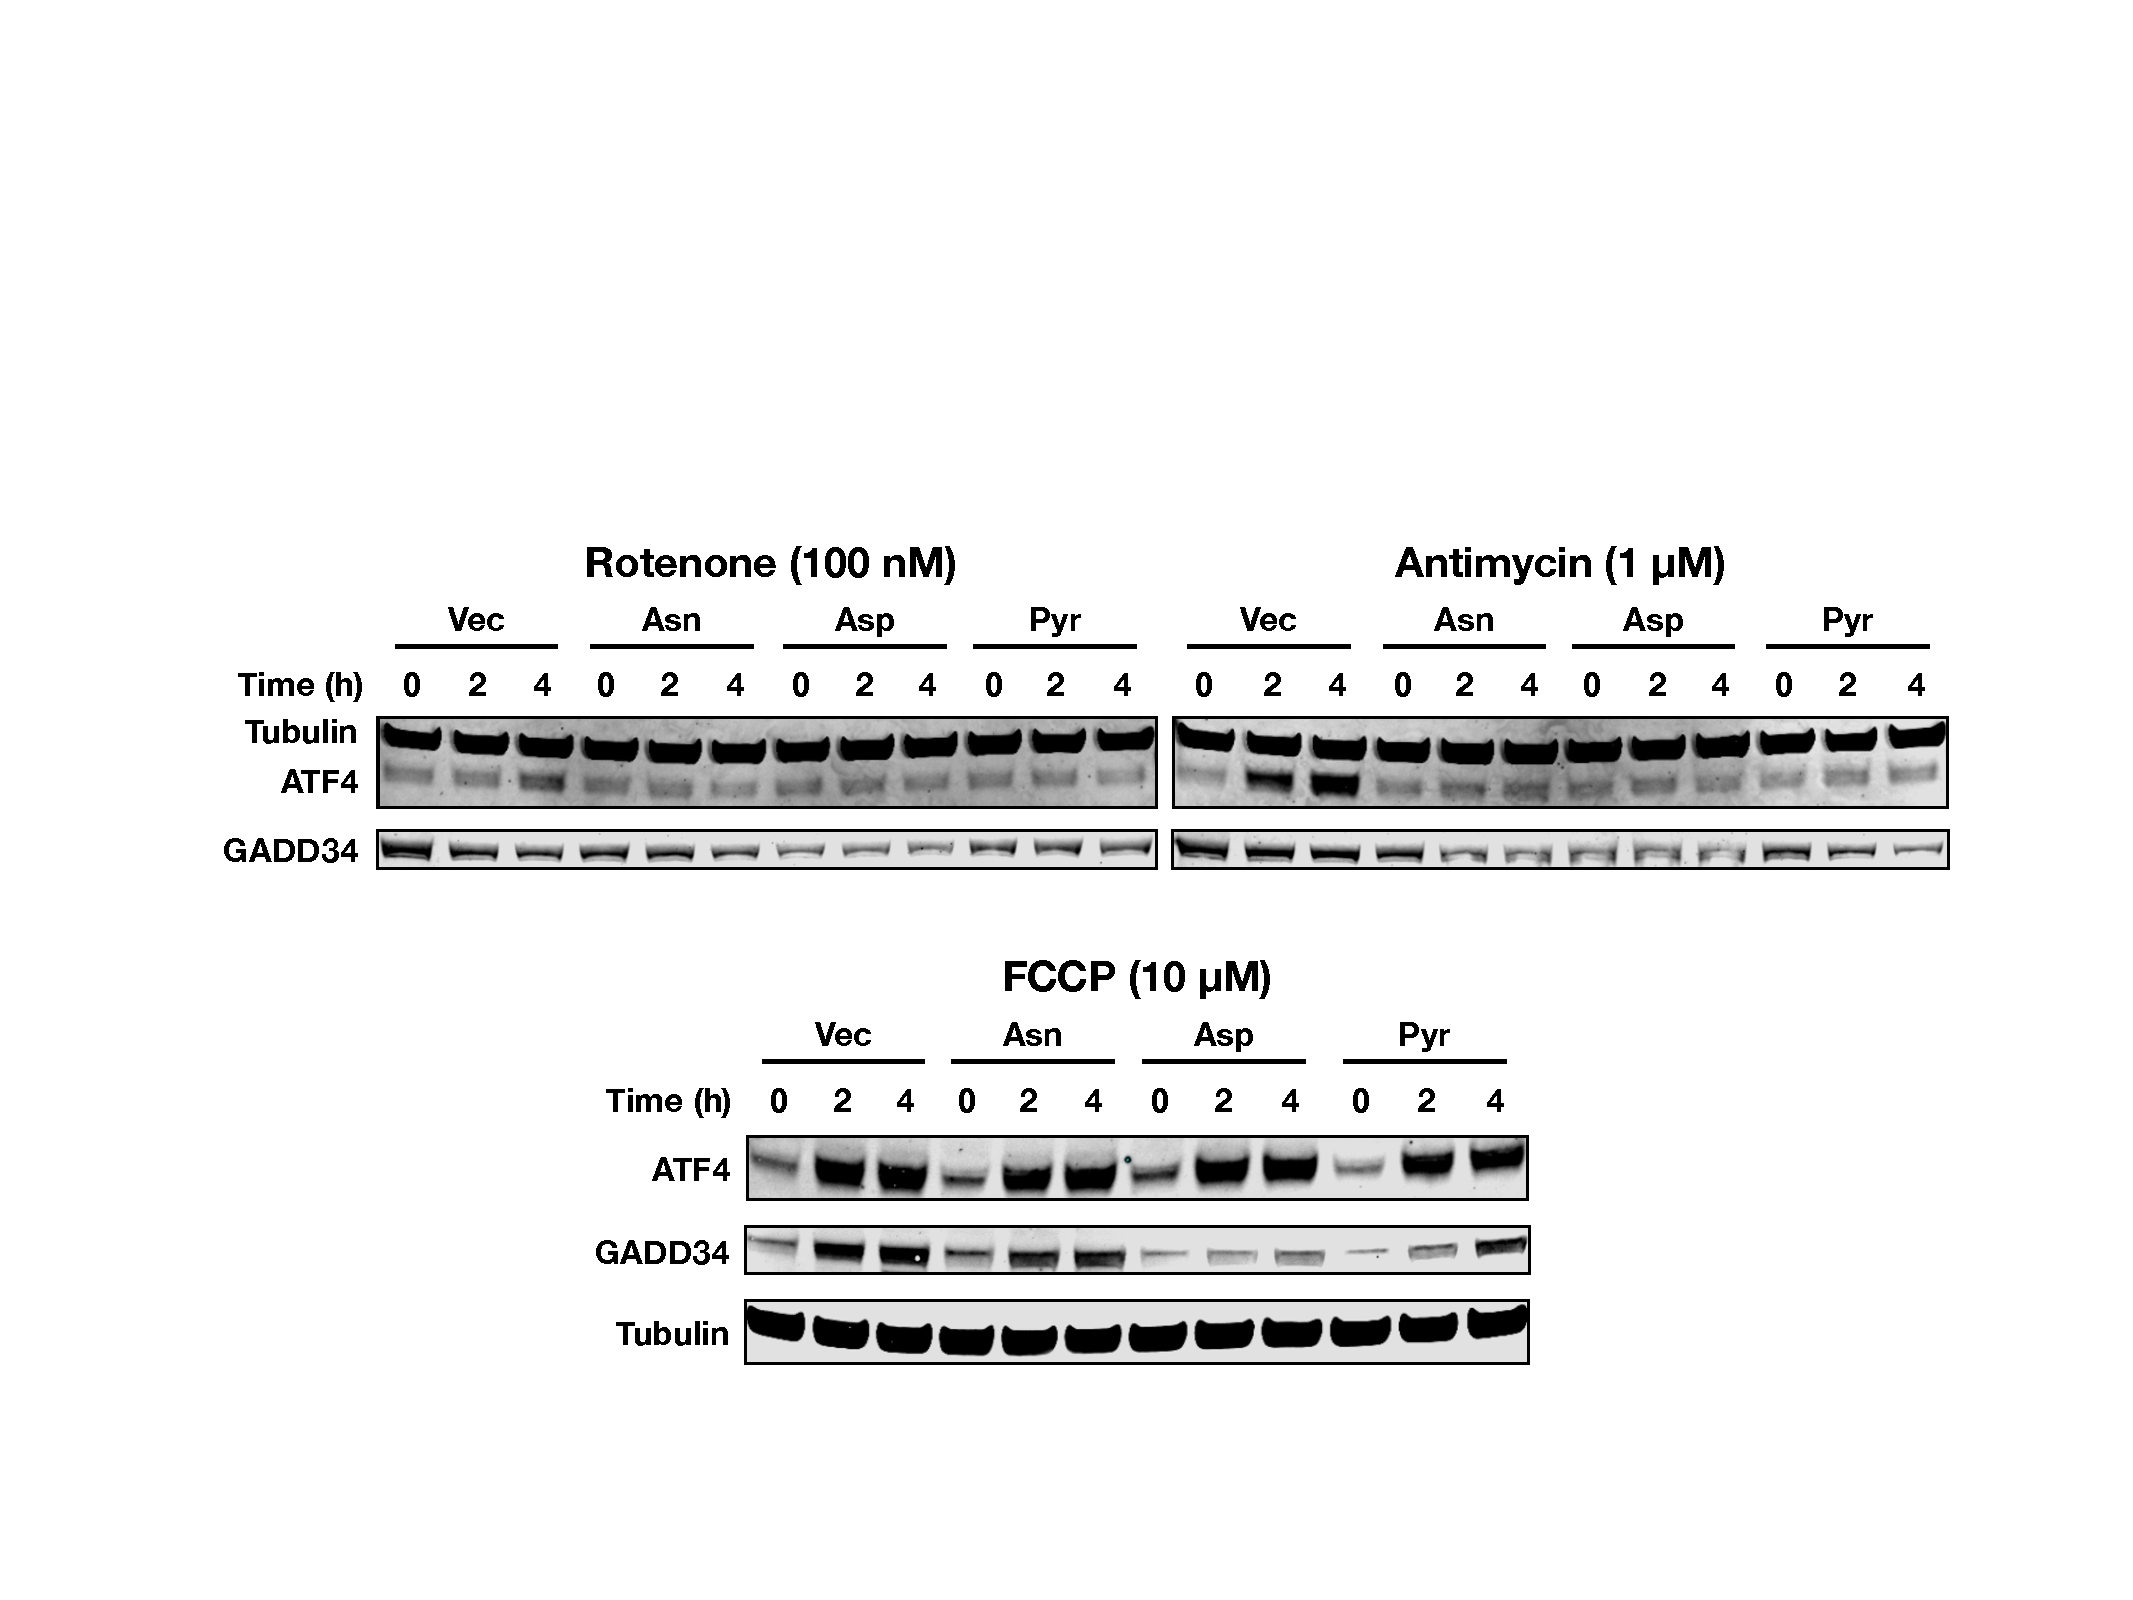
\includegraphics[width=0.95\textwidth]{figures/chap2/app/HT1080_ISR_western.pdf}
    \caption[Mito inhibitor, ATF4 western]{
    Western blot validation of ATF4 reporter in HT1080 cells.
    Treatment and rescue conditions similar to figure \ref{fig:ch2:ISR}.
    % Wednesday 01/12/22
    }
    \label{fig:app_ch2:HT1080_ISR_western}
\end{figure}



\begin{figure}
    \centering
    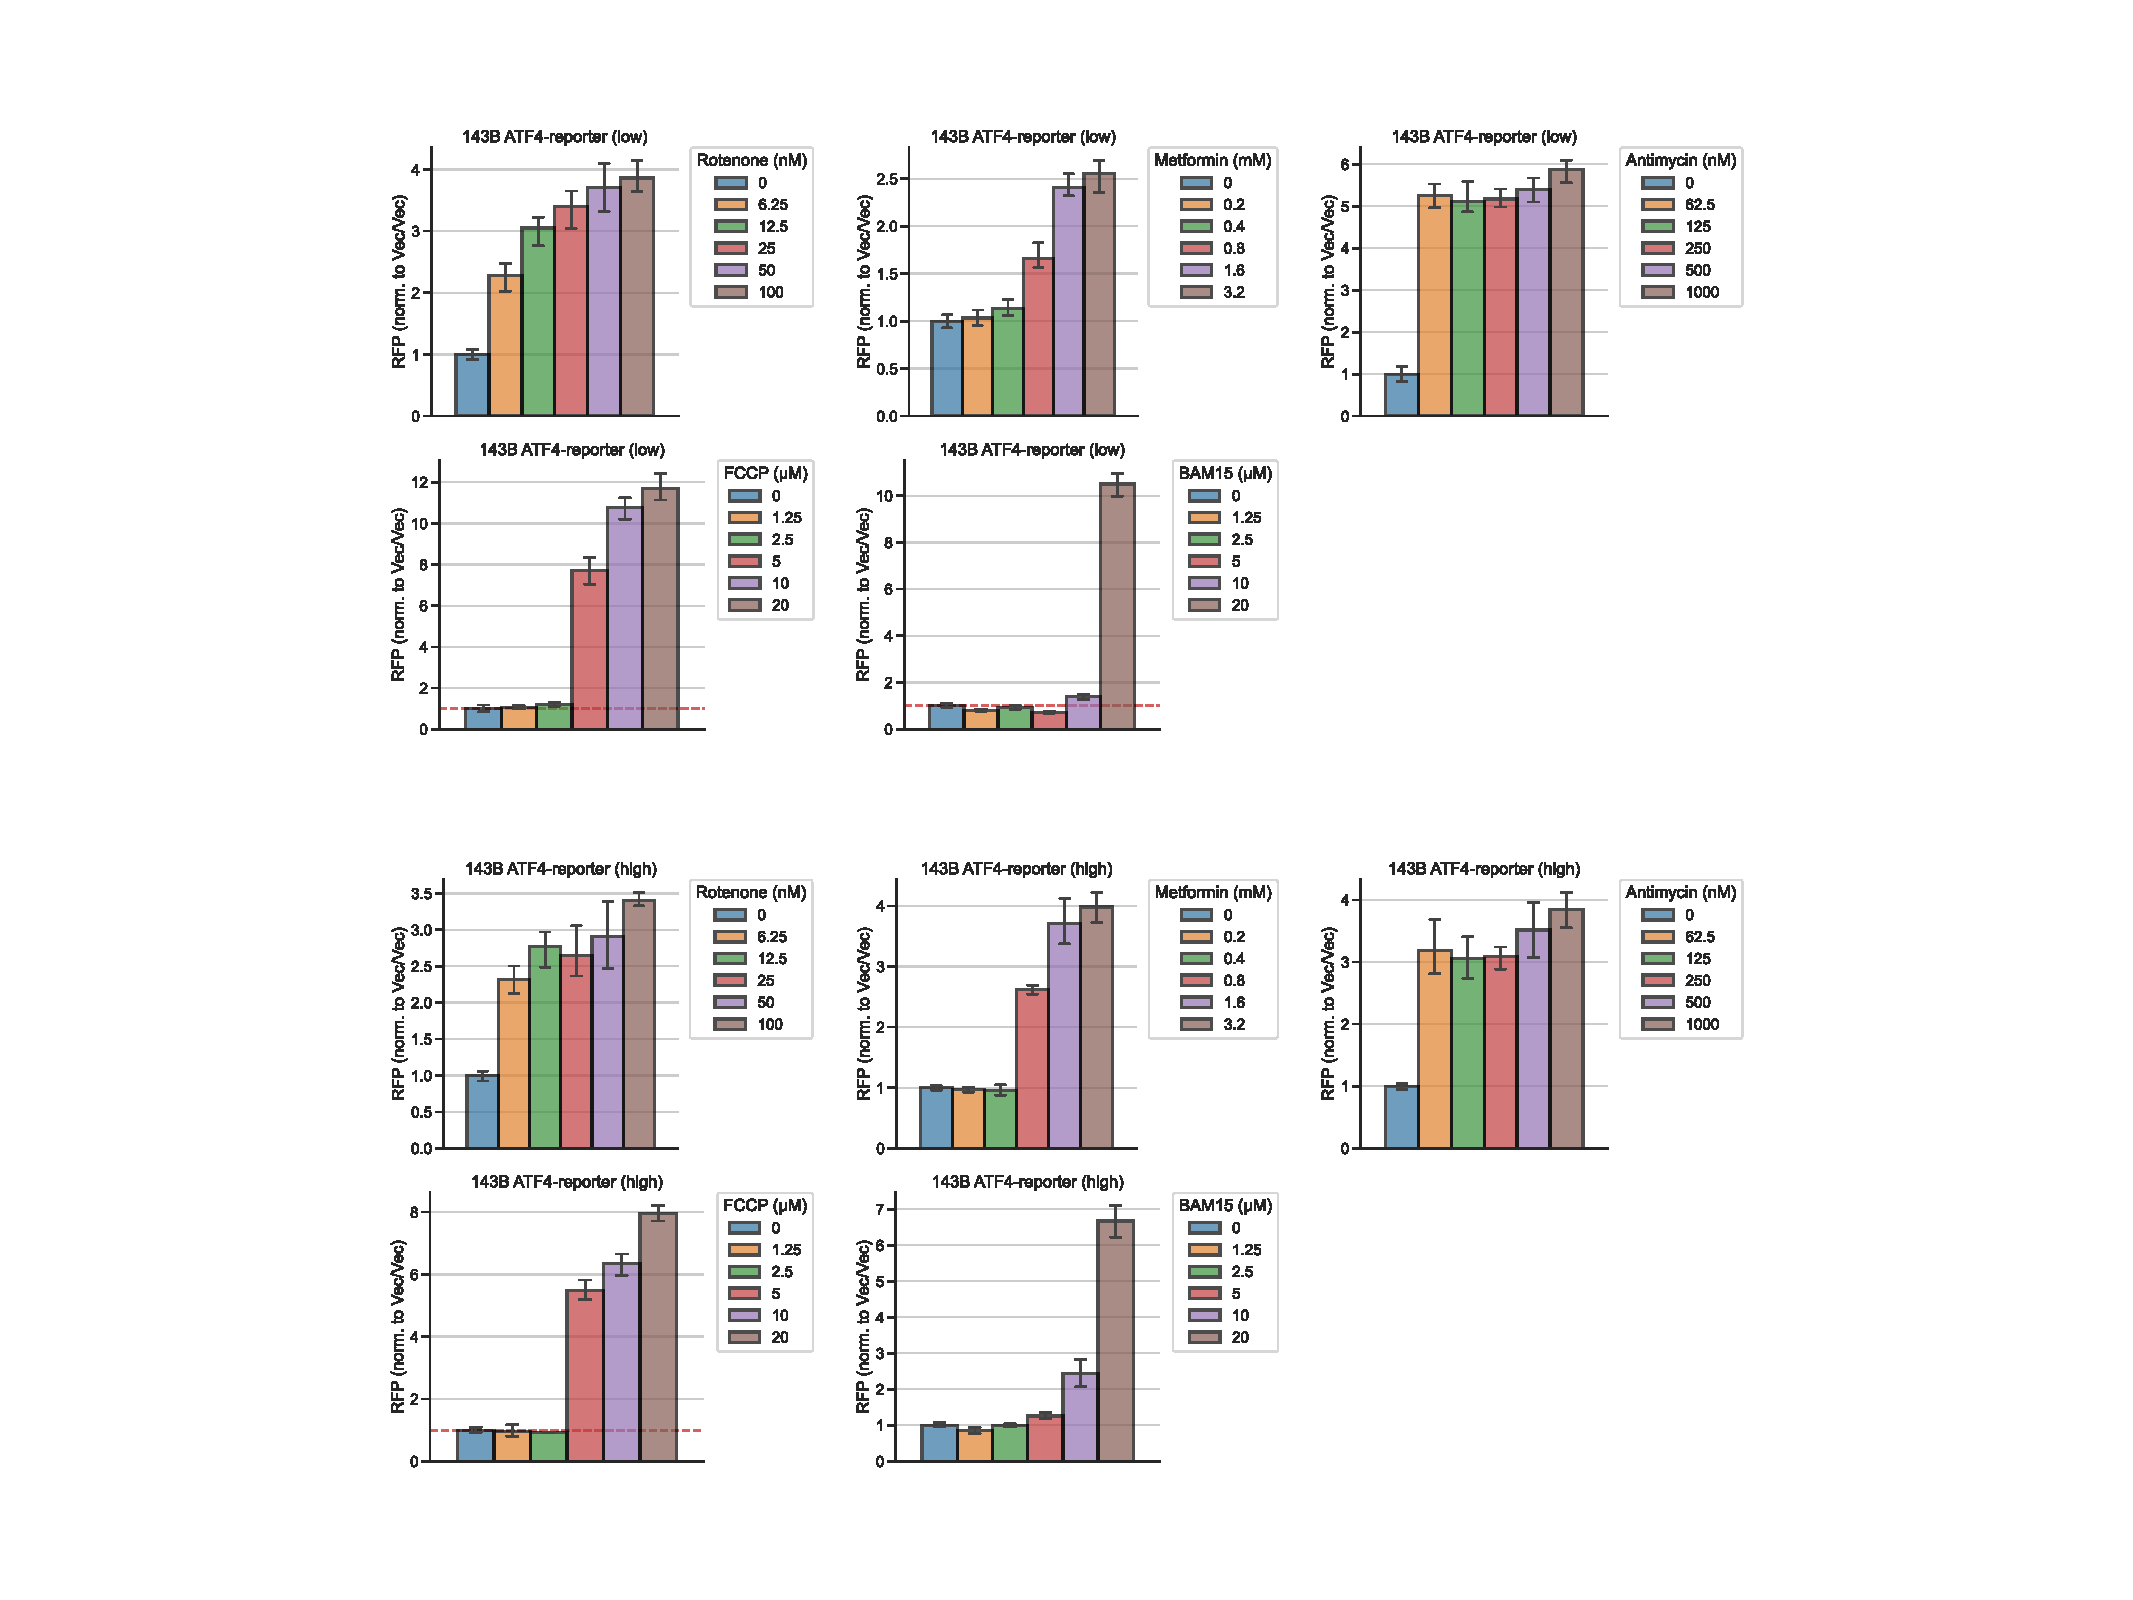
\includegraphics[width=0.95\textwidth]{figures/chap2/app/atf4_ETCtit.pdf}
    \caption[ATF4 reporter, drug titrations]{
    ATF4 reporter, drug titrations.
    ATF4 reporter readout at 17.5 h after drug treatments in 143B cells.
    }
    \label{fig:app_ch2:atf4_ETCtit}
\end{figure}




\begin{figure}
     \centering
     \begin{subfigure}[b]{0.49\textwidth}
         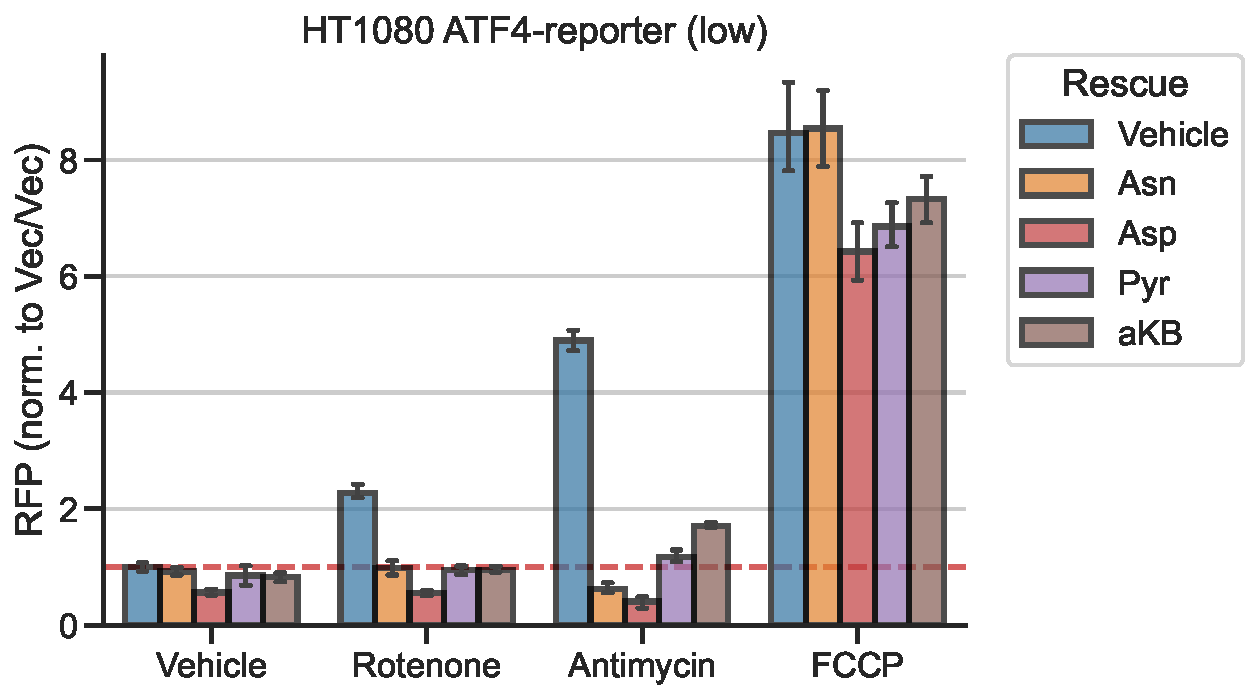
\includegraphics[width=\textwidth]{figures/chap2/app/HT1080_ETCinhib_ATF4rep_low.pdf}
         \caption{}
         \label{fig:app_ch2:HT1080_ETCinhib_ATF4rep_low}
     \end{subfigure}
     \hfill
     \begin{subfigure}[b]{0.49\textwidth}
         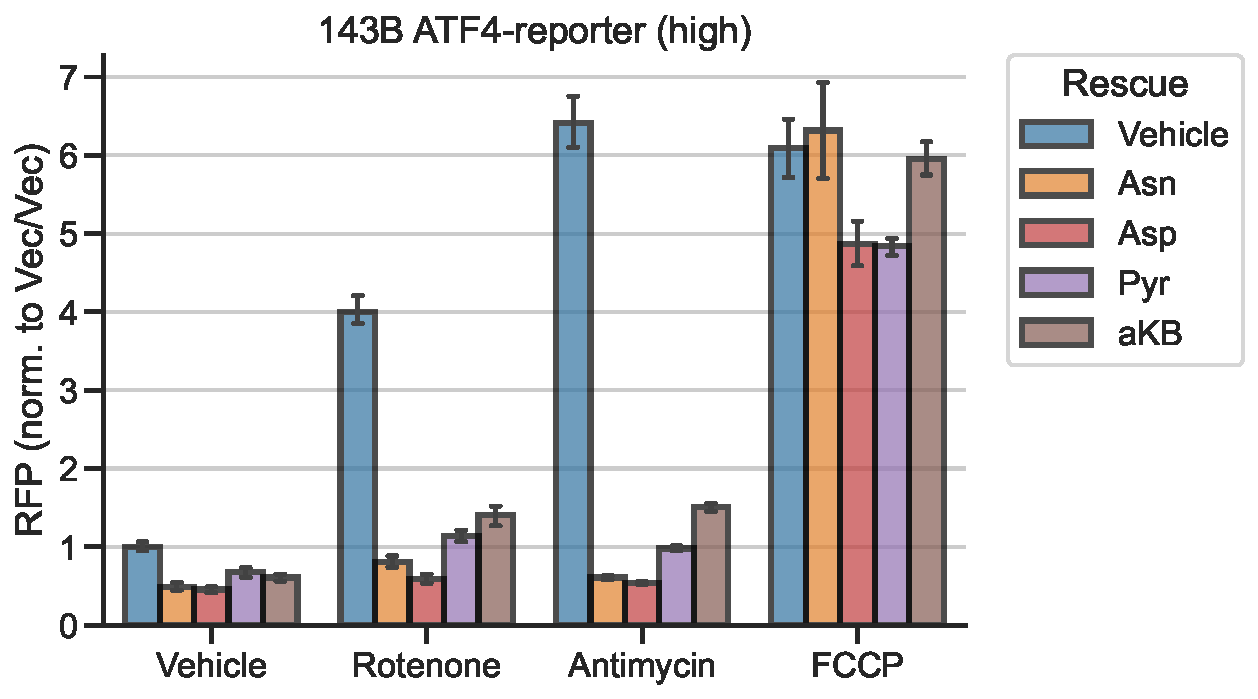
\includegraphics[width=\textwidth]{figures/chap2/app/143B_ETCinhib_ATF4rep_high.pdf}
         \caption{}
         \label{fig:app_ch2:143B_ETCinhib_ATF4rep_high}
     \end{subfigure}
     \hfill
     \begin{subfigure}[b]{0.4\textwidth}
         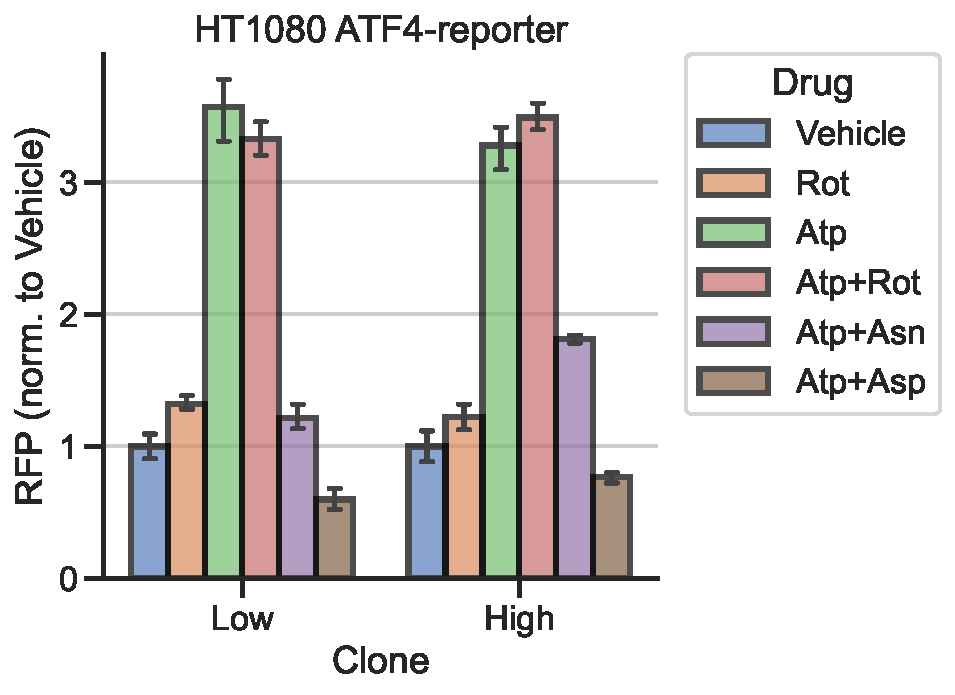
\includegraphics[width=\textwidth]{figures/chap2/app/HT1080_Atp_ATF4rep.pdf}
         \caption{}
         \label{fig:app_ch2:HT1080_Atp_ATF4rep}
     \end{subfigure}
     \hspace{0.06\textwidth}
     \begin{subfigure}[b]{0.4\textwidth}
         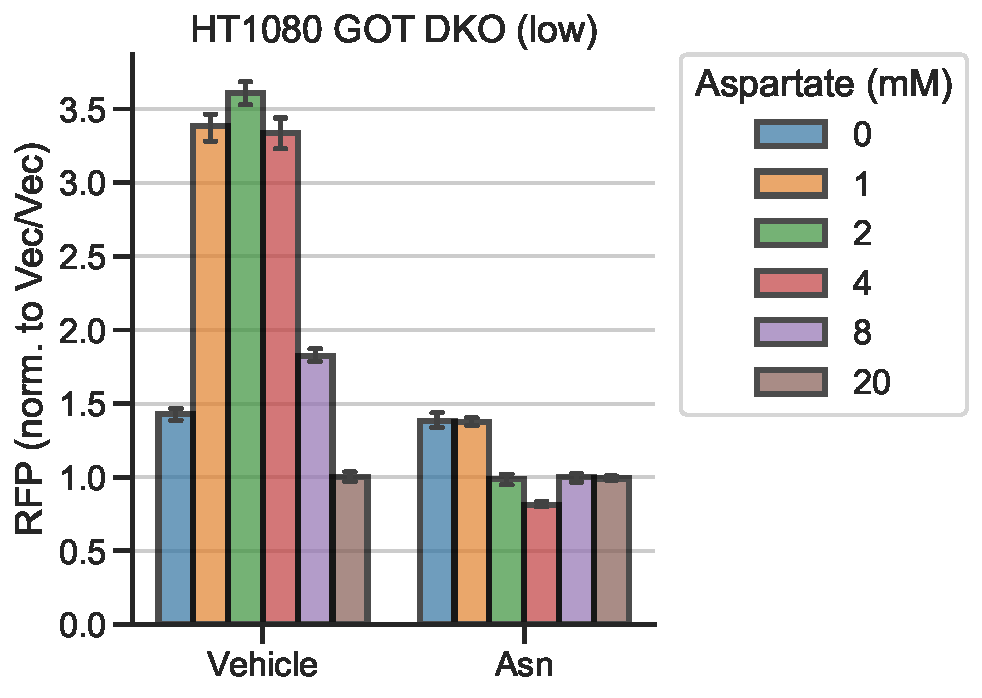
\includegraphics[width=\textwidth]{figures/chap2/app/HT1080_GOT_DKO_Asp_ATF4rep.pdf}
         \caption{}
         \label{fig:app_ch2:HT1080_GOT_DKO_Asp_ATF4rep}
     \end{subfigure}
        \caption[Mito inhibitor induced ATF4 is rescued by Asn, other clones]{
        Related to figure \ref{fig:ch2:ISR}, here showing data generated for other clones.
        (d) Measured 20.5 h after aspartate depletion, Vec/Vec normalization is normalization to the baseline condition (20 mM Asp, no Asn).
        }
        \label{fig:app_ch2:ISR}
\end{figure}




\begin{figure}
    \centering
    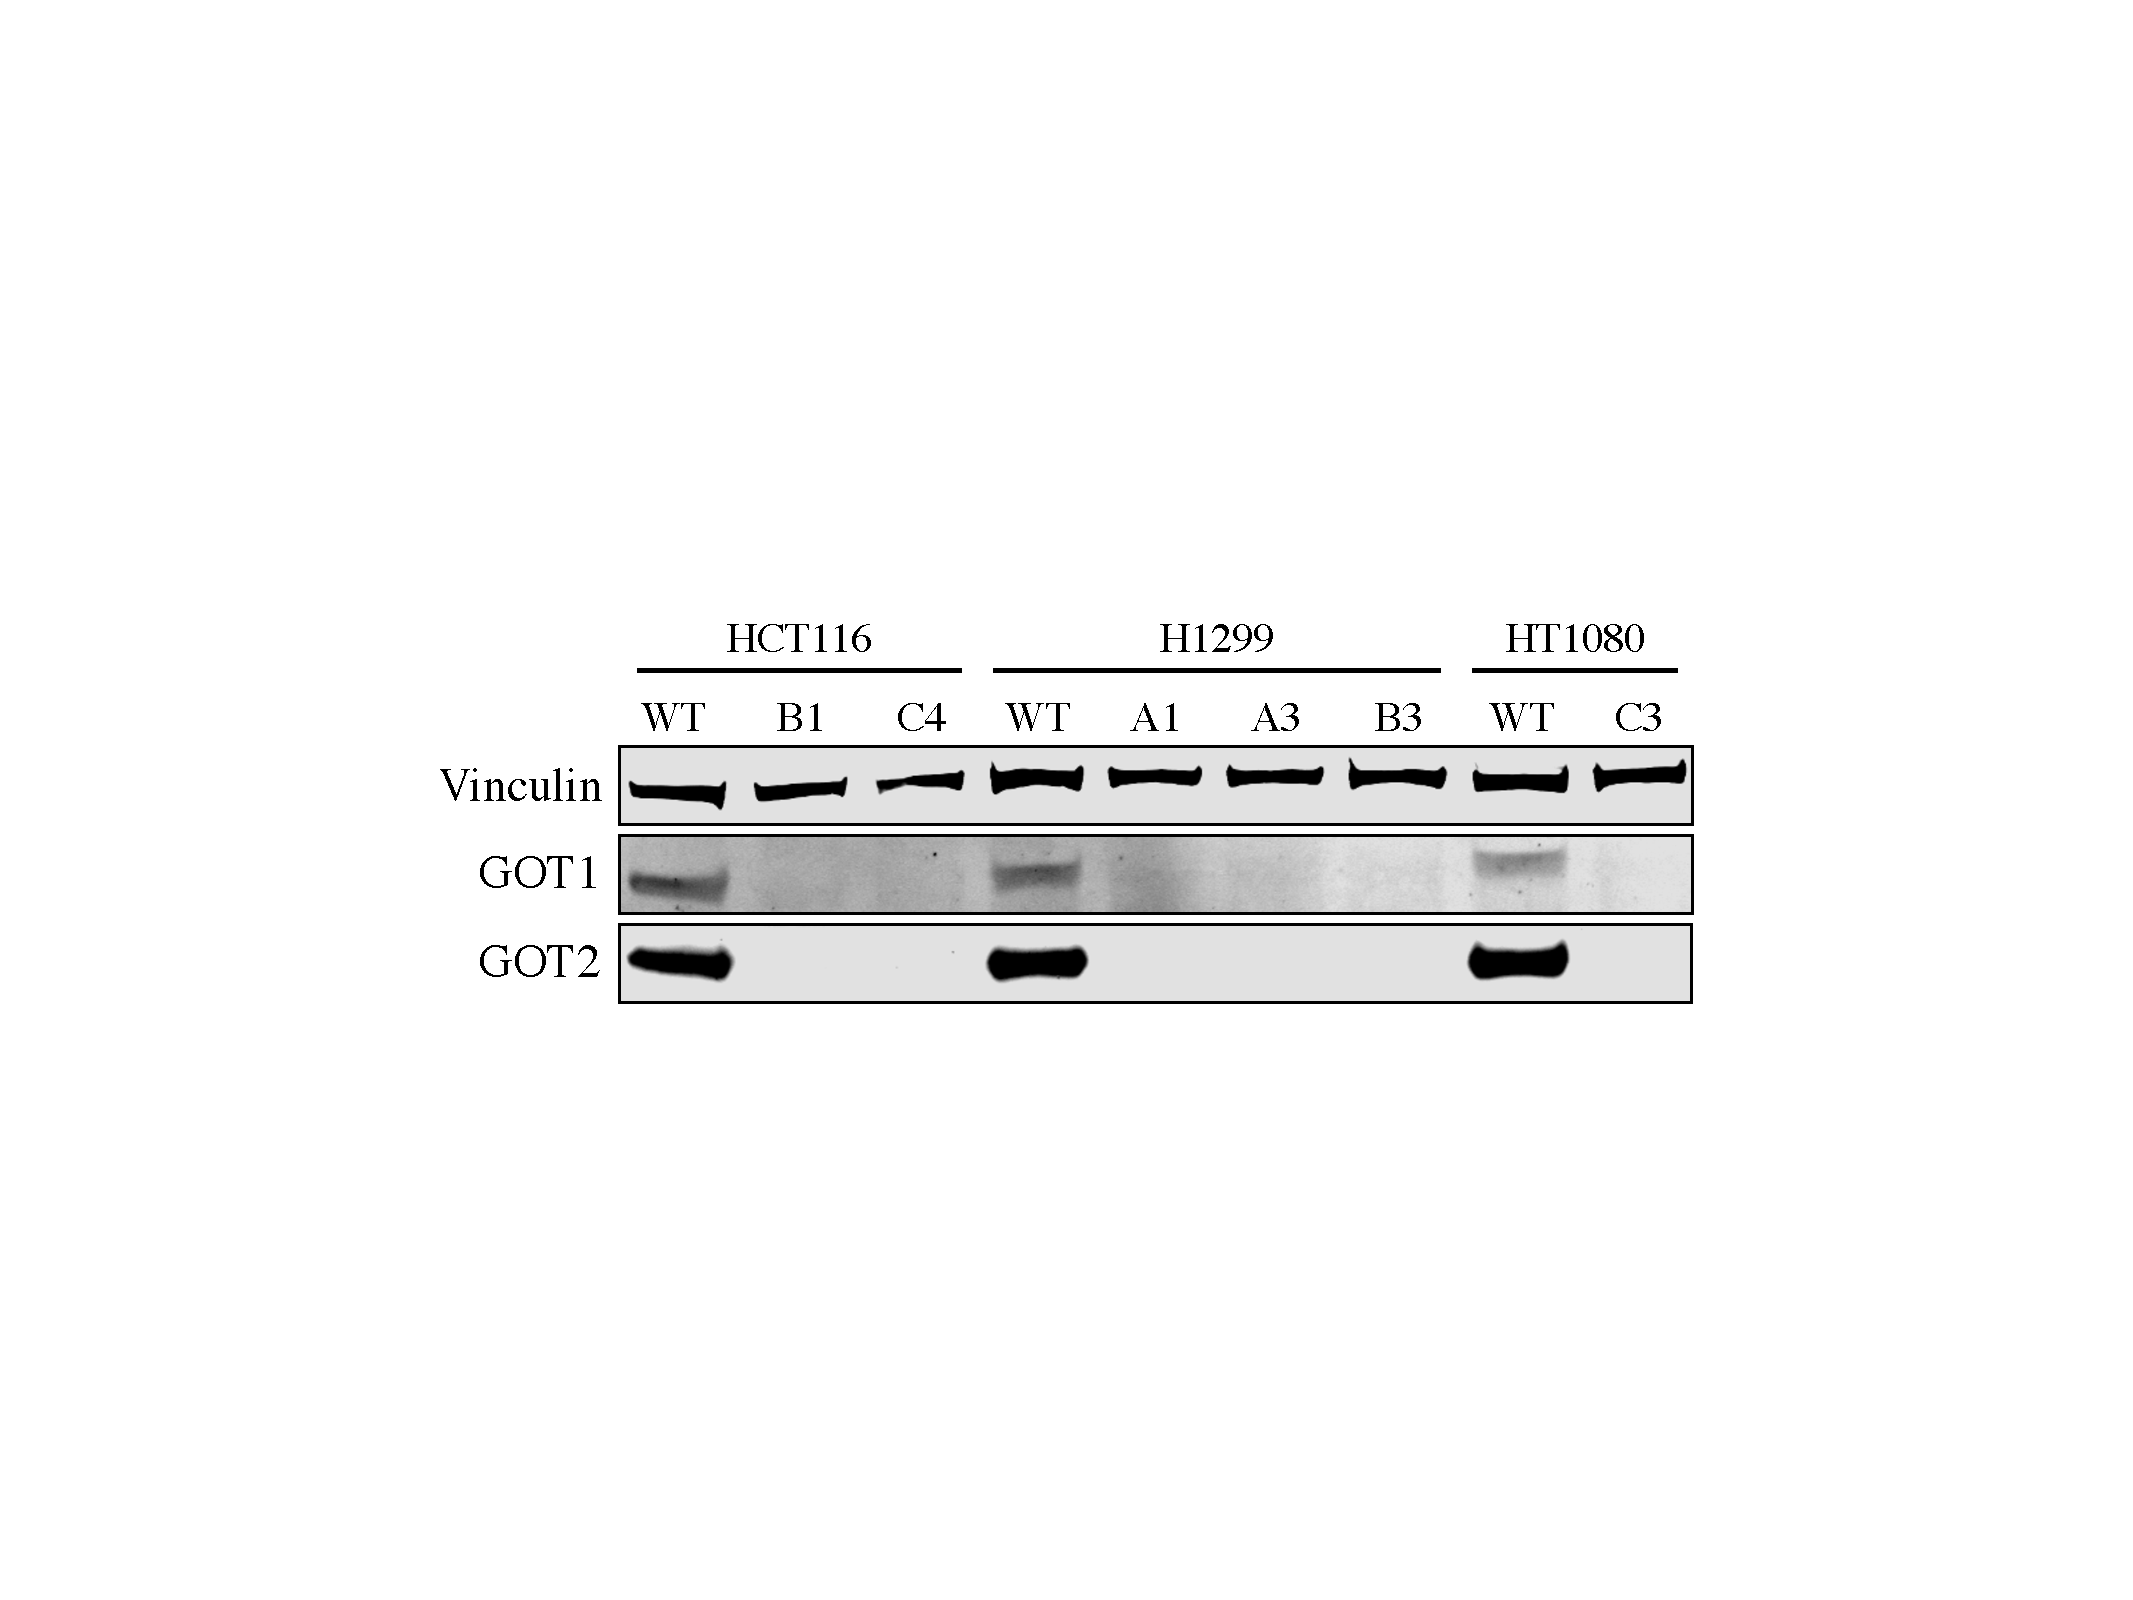
\includegraphics[width=0.55\textwidth]{figures/chap2/app/GOT_DKO_western.pdf}
    \caption[GOT DKO western blot validation]{
    Western blot validation of GOT DKO single cell clones.
    }
    \label{fig:app_ch2:GOT_DKO_western}
\end{figure}








